\documentclass[11pt, margin=1in] {article}
\usepackage [letterpaper, margin=1in]{geometry}
\usepackage{setspace}
\usepackage{cite}
\usepackage{amsmath,amssymb,amsfonts}
\usepackage{algorithm}
\usepackage{algorithmic}
\usepackage{graphicx}
\usepackage{textcomp}
\usepackage{xcolor}
\usepackage{lipsum}
\usepackage{comment}
\usepackage{multirow}
\usepackage{subcaption}
\newcommand{\argmax}[1]{\underset{#1}{\operatorname{arg}\operatorname{max}}\;}
\usepackage{listings}
\usepackage{xcolor}
\usepackage{ragged2e}
\usepackage{longtable}
\usepackage{lscape}
\usepackage{tabularx}
\usepackage{sectsty}
%\sectionfont{\fontsize{12}{15}\selectfont}
%\subsectionfont{\fontsize{11}{12}\selectfont}
\lstset { %
	language=C++,
	backgroundcolor=\color{black!5}, % set backgroundcolor
	basicstyle=\footnotesize,% basic font setting
}
\usepackage[titletoc,title]{appendix}
\usepackage{tikz}
\usetikzlibrary{shapes.geometric, arrows}
\usepackage{hyperref}
\hypersetup{
	colorlinks=true,
	linktoc=all,
	linkcolor=blue
}
\title{A DSL to Automate Initial and Exploratory Analysis for Regression-Based Data Analytics Projects}
\author{Sayed Ahmed and Sepehr Bayat \footnote{(alphabetical order)}}
\date{}
\begin{document}
\maketitle
\tableofcontents
\section{Abstract}
Model Driven Development (MDD) can facilitate faster software development while providing consistency and protecting code integrity. Domain Specific Languages utilizing MDD can simplify the development of a specific set of repetitive tasks for a particular aspect and domain. In machine learning and data analytics projects, several tasks such as data cleaning, data adjustment, Exploratory Data Analysis (EDA), and Initial Data Analysis (IDA) are common for most projects. Although the extent and need can vary,  the code for several  aspects can be made the same to avoid repetitive code and tasks. Hence, in this project, we have developed a Domain Specific Language utilizing MDD. We have developed a Domain Specification Language (DSL) to automate Initial and Exploratory Analysis for Regression-Based Data Analytics Projects. Our project automates and writes code for Data Cleaning, Initial Analysis, and Exploratory Data Analysis. Anyone wanting to write a Data Analytics Project can use this DSL. The user can use a GUI or Text Format to define data sources and relationships among data sources. Relationships can be selected from predefined selections. The developer can select the types of analysis he or she wants such as clean/replace null values, unitary analysis, unitary plots, bi-variate regression, bi-variate plots, and r-square calculation. The DSL, by default, can/will generate code for a pre-configured (default configuration) set of tasks where the developer does not want to provide a custom list of tasks. Mandatory requirements are that our DSL will write code to clean/replace null/missing values, align data type to the majority type, r-square/adjusted r-square calculation, data normalization, unitary plot, bi-variate plot, bi-variate regression plot with the target.

%Data Analytics Regression Projects have some common tasks such as Data Cleaning, Initial Analysis, and Exploratory Data Analysis to be conducted.


\section{Introduction}

\textbf{Tools to Use}
\begin{itemize}
	\item Emfatic/Ecore
	\item Eugenia
\begin{itemize}
	\item Xtext in Eugenia 
\end{itemize}
	\item Papyrus (UML tool)
	
	\item Probably: Model querying (EOL)
	\item Probably: Model validation (EVL)

\end{itemize}
\section{Related Work}

\section{Proposed Solution}

\subsection{Methodology Overview}

\subsection{Overall Steps}
To develop the DSL, the steps that we followed are:
\begin{enumerate}
	\item Develop a Metamodel for the DSL to automate Data Cleaning/EDA/IDA
		\begin{itemize}
			\item Define the abstract - syntax i.e. define the terminology: Abstract Syntax
			\item Create/define Concrete Syntax: Relationship/Symbols utilizing the Abstract Syntax
			\item Define the semantic syntax
		\end{itemize}
	\item Develop Model: Models are instances of Meta Models
	\item Develop UI/Editor for the developer (use GMF, Eugenia): GMF/Graphical UI to write program.
	\item Model to code % (I need to think again why I thought it when I thought it first)
\end{enumerate}

\flushleft \justify While creating the Meta Models we will define some rules so that it can verify the validity of the metamodel. These rules will verify the flow and steps that developers use for a project. We may provide developers the facility to create a state diagram to define the steps of the code flow. These rules can verify the validity of such state flow diagrams.

\flushleft \justify We will use Eclipse Ecore, and EMFatic for creating Meta Models. We also have come across tools from Microsoft as part of Visual Studio that is also an option to utilize.

\subsection{Artefacts of our DSL}
Our DSL can result in the following outputs:

\begin{enumerate}
	\item Null Value Replaced Data
	\item Missing Value Replaced Data
	\item Rescaled, harmonized, and Normalized data
	\item R-Square Analysis with P-values and F-Significance
	\item Visualizations for Unitary, Bi-Variate, and multivariate analysis
	\item Correlation plots (Pearson, Spearman, Kendall Tau Coeff)			
\end{enumerate}

\flushleft \justify Overall, the output will have data, code, and visualizations. As an example, our DSL can provide some features like excel plugins named XL-STAT, and Data Analysis Toolpak. However, we will generate code as well that developers will be able to modify.

\flushleft \justify Output/Artefacts in Chronological Order:
\begin{enumerate}
	\item Null Value Replaced Data
	\item Missing Value Replaced Data
	\item Rescaled, harmonized, and Normalized data
	\item Visualizations for Unitary, Bi-Variate, and multivariate analysis
	\item R-Square Analysis with P-values and F-Significance
	\item P-value, F-significance, and some comments: important/not-important factors/Variables.
	\item Correlation plots (Pearson, Spearman, Kendall Tau Coeff)
\end{enumerate}

\subsection {Models and State Diagrams}
\flushleft \justify From the meta-model, models can be created. Developers will have the facility to create models based on the meta-model. Developers will create the models using abstract, and concrete syntax. We have provided primarily text-based Model creation. However, graphics based model creation is an option as well.

\flushleft \justify Potential models that developers might be able to create are as follows:

\begin{itemize}
	\item NullMissingModel
	\item ScaleModel
	\item NormalizeModel
	\item StandardizeModel
	\item VisualPlotModel with Unary/Binary/Multi Sub Models
	\item RSquareModel
	\item PValueFSignificanceModel
\end{itemize}


\flushleft \justify Developers will have the option to create a state flow diagram that will utilize the model to define the work/code-generation flow they want. State diagrams will contain conditional/decisional flows. 


\subsection{Meta Model Details}
\flushleft \justify A diagram of our meta model is provided in the figure ~\ref{data-curation-meta-model}. Meta Model Details are provided below:

\begin{figure}[!htb]
\begin{tabular}{c}
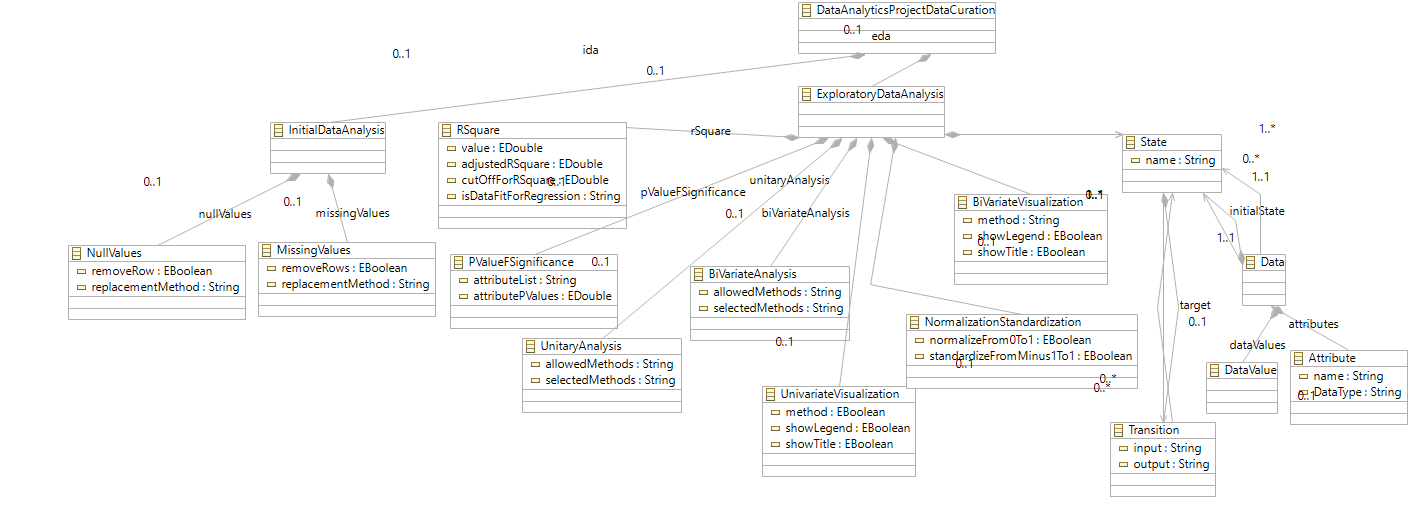
\includegraphics[scale=0.5]{images/meta-model-ecore-diagram.png} \\
\end{tabular}
\caption{Data Curation Meta Model}
\label{data-curation-meta-model}
\end{figure}


\textbf{Abstract Syntax}
\begin{itemize}
	\item Null
	\item Missing
	\item RSquare
	\item PF
	\item UVisualize
	\item BiVisualize
\end{itemize}


\textbf{Concrete  Syntax Elements}
\begin{itemize}
	\item Box: Model
	\item Circle: Process
	\item Rhombus: Start and End.
	\item Directed arrow: flow
\end{itemize}

\textbf{Symantic  Syntax Elements}
\begin{itemize}
	\item to be filled
\end{itemize}

\textbf{Meta Model Rules}:
\begin{itemize}
	\item No visualizations before Normalization/Standardization unless excepted
	\item All independent features will need to be numeric, else drop/convert
	\item Target feature will need to be numeric
\end{itemize}

\textbf{Meta Model Need and Approaches}:
\flushleft \justify Do we need metamodels? or we can just directly start with Models? Because of the context, applications will have varying needs for Data Cleaning, EDA, and IDA hence, Metal Model will be advantageous to support these varieties. Meta models will provide the flexibility to extend this project to other areas such as Natural Language Processing (NLP), Classification, and Clustering projects. Meta-models can help in one of two approaches such as one as we mentioned that models can be created for Regression, Classification, Clustering, and NLP projects; another way metal models help is: among all the functionalities/codes/features that meta-models will provide, a project can choose to use a sub-set of them; hence, creating a variation of the models. Hence, meta-models will be important. Selection can be automated or developer selected.

\flushleft \justify Regression, Classifications, clustering, and NLP all need EDA/IDA; hence, metal-models can bring the common EDA/IDA features/code into the meta models. 

\flushleft \justify Similarity:
\flushleft \justify Musicians: Characteristics  and variations
\flushleft \justify EDA/IDA: Models with varying characteristics. We can create variations.


\subsection{EMFatic Meta Model: Abstract Syntax}

Class EDA \{
\begin {itemize}
	\item attr name: string
	\item attr style: style-category
	\item Null
	\item Missing
	\item  Normal
	\item Scale
	\item standard
	\item unary
	\item binary		
\end{itemize}
\}


Class NULL \{
\begin {itemize}
	\item attr name: string
		
\end{itemize}
\}

Class Normal \{
\begin {itemize}
	\item attr name: string
		
\end{itemize}
\}



enum style-category \{
\begin {itemize}
	\item attr name: string
		
\end{itemize}
\}


\subsection{Models from EMFatic Meta Model}


Class EDA-REG \{
\begin {itemize}
	\item attr name: string
		
\end{itemize}
\}


Class IDA-REG \{
\begin {itemize}
	\item attr name: string
		
\end{itemize}
\}


\subsection{Graphical Concrete Syntax Example}
\begin{figure} [!htb]
\begin{tabular}{|c|}
\hline
Data\\
\hline
Null Replace\\
\hline
Scale\\
\hline

\end{tabular}
\end{figure}


\begin{figure} [!htb]
\begin{tabular}{|c|}
\hline
Data\\
\hline
Null Replace\\
\hline
Scale\\
\hline
Unary Visual\\
\hline
R-Square\\
\hline
\end{tabular}
\end{figure}

\vspace{1in}

\subsection{Screenshots of Metamodels from ongoing implementation}
Provided in figure ~\ref{metamodelcode}
\begin{figure}[!htb]
\begin{tabular}{|c|c|}
\hline
 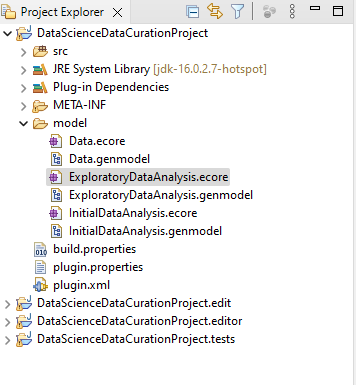
\includegraphics[scale=0.5]{images/code/models-and-code.png} & 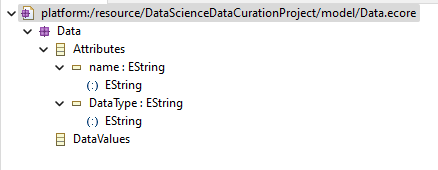
\includegraphics[scale=0.5]{images/code/data-ecore-model.png} \\
\hline
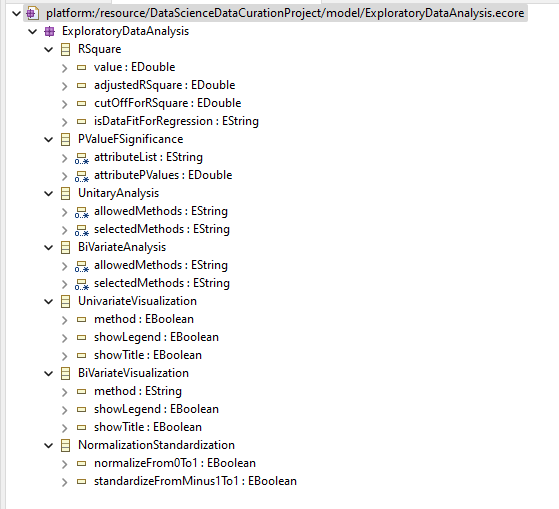
\includegraphics[scale=0.5]{images/code/eda-ecore-model.png} & ...\\
\hline
\end{tabular}
\caption{Screenshots of Metamodels from ongoing implementation}
\label{metamodelcode}
\end{figure}



\subsection{Flow IDA/EDA in a Diagram}
\tikzstyle{startstop} = [rectangle, rounded corners, minimum width=2cm, minimum height=1cm,text centered, draw=black, fill=red!30]
\tikzstyle{io} = [trapezium, trapezium left angle=70, trapezium right angle=110, minimum width=2cm, minimum height=1cm, text centered, draw=black, fill=blue!30]
\tikzstyle{process} = [rectangle, minimum width=3cm, minimum height=1cm, text centered, draw=black, fill=orange!30]
\tikzstyle{decision} = [diamond, minimum width=3cm, minimum height=1cm, text centered, draw=black, fill=green!30]
\tikzstyle{arrow} = [thick,->,>=stealth]
\begin{figure}[!htb]
\begin{tabular}{c}
\begin{tikzpicture}[node distance=1.5cm]
<TikZ code>
\node (start) [startstop] {Start};

\node (stop) [startstop] {Stop};

\end{tikzpicture}
\end{tabular}
\caption{Flow EDA/IDA}
\label{Flow EDA/IDA}
\end{figure}

\subsection{UI Editor}
\flushleft \justify Use GMF/Eugenia to create the editor (make use of .gmfgen and .diagram files)
% ''Then, a model-to-text transformation consumes the .gmfgen model and produces a new plug-in project (.diagram) that contains the Java code for the diagram-based editor'' GMF Slide
\flushleft \justify From class notes: ''• Once the .gmfgraph, .gmftool, and .gmfmap models are in place, GMF provides a model-to- model transformation that creates a generator model from them (.gmfgen)''


%\flushleft \justify Eugenia: A tool that simplifies the development of GMF-based editors
%\flushleft \justify ''  Generating the Diagram-based Editor
%\flushleft \justify • Once the .gmfgraph, .gmftool, and .gmfmap models are in place, GMF provides a model-to- model transformation that creates a generator model from them (.gmfgen)
%\flushleft \justify – Provides additional customization options for the editor
%\flushleft \justify • Then, a model-to-text transformation consumes the .gmfgen model and produces a new plug-in project (.diagram) that contains the Java code fo the diagram-based editor
 ''



%********************************

%\tikzstyle{startstop} = [rectangle, rounded corners, minimum width=2cm, minimum height=1cm,text centered, draw=black, fill=red!30]
%\tikzstyle{io} = [trapezium, trapezium left angle=70, trapezium right angle=110, minimum width=2cm, minimum height=1cm, text centered, draw=black, fill=blue!30]
%\tikzstyle{process} = [rectangle, minimum width=3cm, minimum height=1cm, text centered, draw=black, fill=orange!30]
%\tikzstyle{decision} = [diamond, minimum width=3cm, minimum height=1cm, text centered, draw=black, fill=green!30]
%\tikzstyle{arrow} = [thick,->,>=stealth]
%
%\subsection{Overall Architecture}
%~\ref{overall-architecture}.
%\begin{figure}[!htb]
%\begin{tabular}{c}
%\begin{tikzpicture}[node distance=1.5cm]
%<TikZ code>
%\node (start) [startstop] {Start};
%\node (surveydata) [io, text width=8cm, below of=start] {CDC/NHANES Survey data on Demographics, Dietary Intake, and ACR results };
%\node (acrdata) [io, text width=2.5cm, below of=surveydata, yshift=-0.25cm, xshift=-3cm] {ACR Data};
%\node (fooditems) [io, text width=2cm, right of=acrdata, xshift=5cm] {Food Items};
%\node (foodgroups) [io, text width=4cm, below of=fooditems] {Food Group Intake};
%
%\node (proceefoodacr) [process, text width=4cm, below of=acrdata] {Merge ACR, Food Group Intake};
%\node (sourcefood) [io, text width=4cm, below of=proceefoodacr] {Source: Food Group Intake Target: ACR};
%\node (cluster) [process, text width=5cm, below of=sourcefood] {Clustered Groups based on Age and AC level};
%\node (regression) [process, text width=5cm, below of=cluster, yshift=-0.25cm] {Regression/Correlation Relate Food Groups with ACR};
%\node (corregression) [io, text width=3cm, below of=regression, xshift=-2cm, yshift = -1cm] {Correlated Food Groups with ACR};
%\node (ml) [process, right of=corregression, xshift=3cm] {ML Methods};
%\node (acrpredict) [process, text width=5cm, below of=ml] {ACR Predictability};
%\node (predicted) [io, text width=3cm, below of=acrpredict, xshift=-2cm] {Predicted ACR from Food Intake};
%\node (stop) [startstop, below of=predicted] {Stop};
%
%
%
%\draw [arrow] (start) -- (surveydata);
%\draw [arrow] (surveydata) -- (acrdata);
%\draw [arrow] (surveydata) -- (fooditems);
%\draw [arrow] (fooditems) -- (foodgroups);
%
%\draw [arrow] (acrdata) -- (proceefoodacr);
%\draw [arrow] (foodgroups) -- (proceefoodacr);
%
%\draw [arrow] (proceefoodacr) -- (sourcefood);
%\draw [arrow] (sourcefood) -- (cluster);
%\draw [arrow] (cluster) -- (regression);
%\draw [arrow] (regression) -- (corregression);
%\draw [arrow] (regression) -- (ml);
%
%\draw [arrow] (ml) -- (corregression);
%\draw [arrow] (ml) -- (acrpredict);
%\draw [arrow] (acrpredict) -- (predicted);
%\draw [arrow] (predicted) -- (stop);
%\end{tikzpicture}
%\end{tabular}
%\caption{Example Architecture Diagram}
%\label{overall-architecture}
%\end{figure}



\section{Experiments Changed}

\section {Results and Discussion}

\section{Conclusion}


\subsection{Future Work}

%\section{References}

\begin{thebibliography}{1}



\end{thebibliography}
\pagebreak
\section{Appendix}

%\begin{figure}
\begin{tabular}{|c|}
\hline
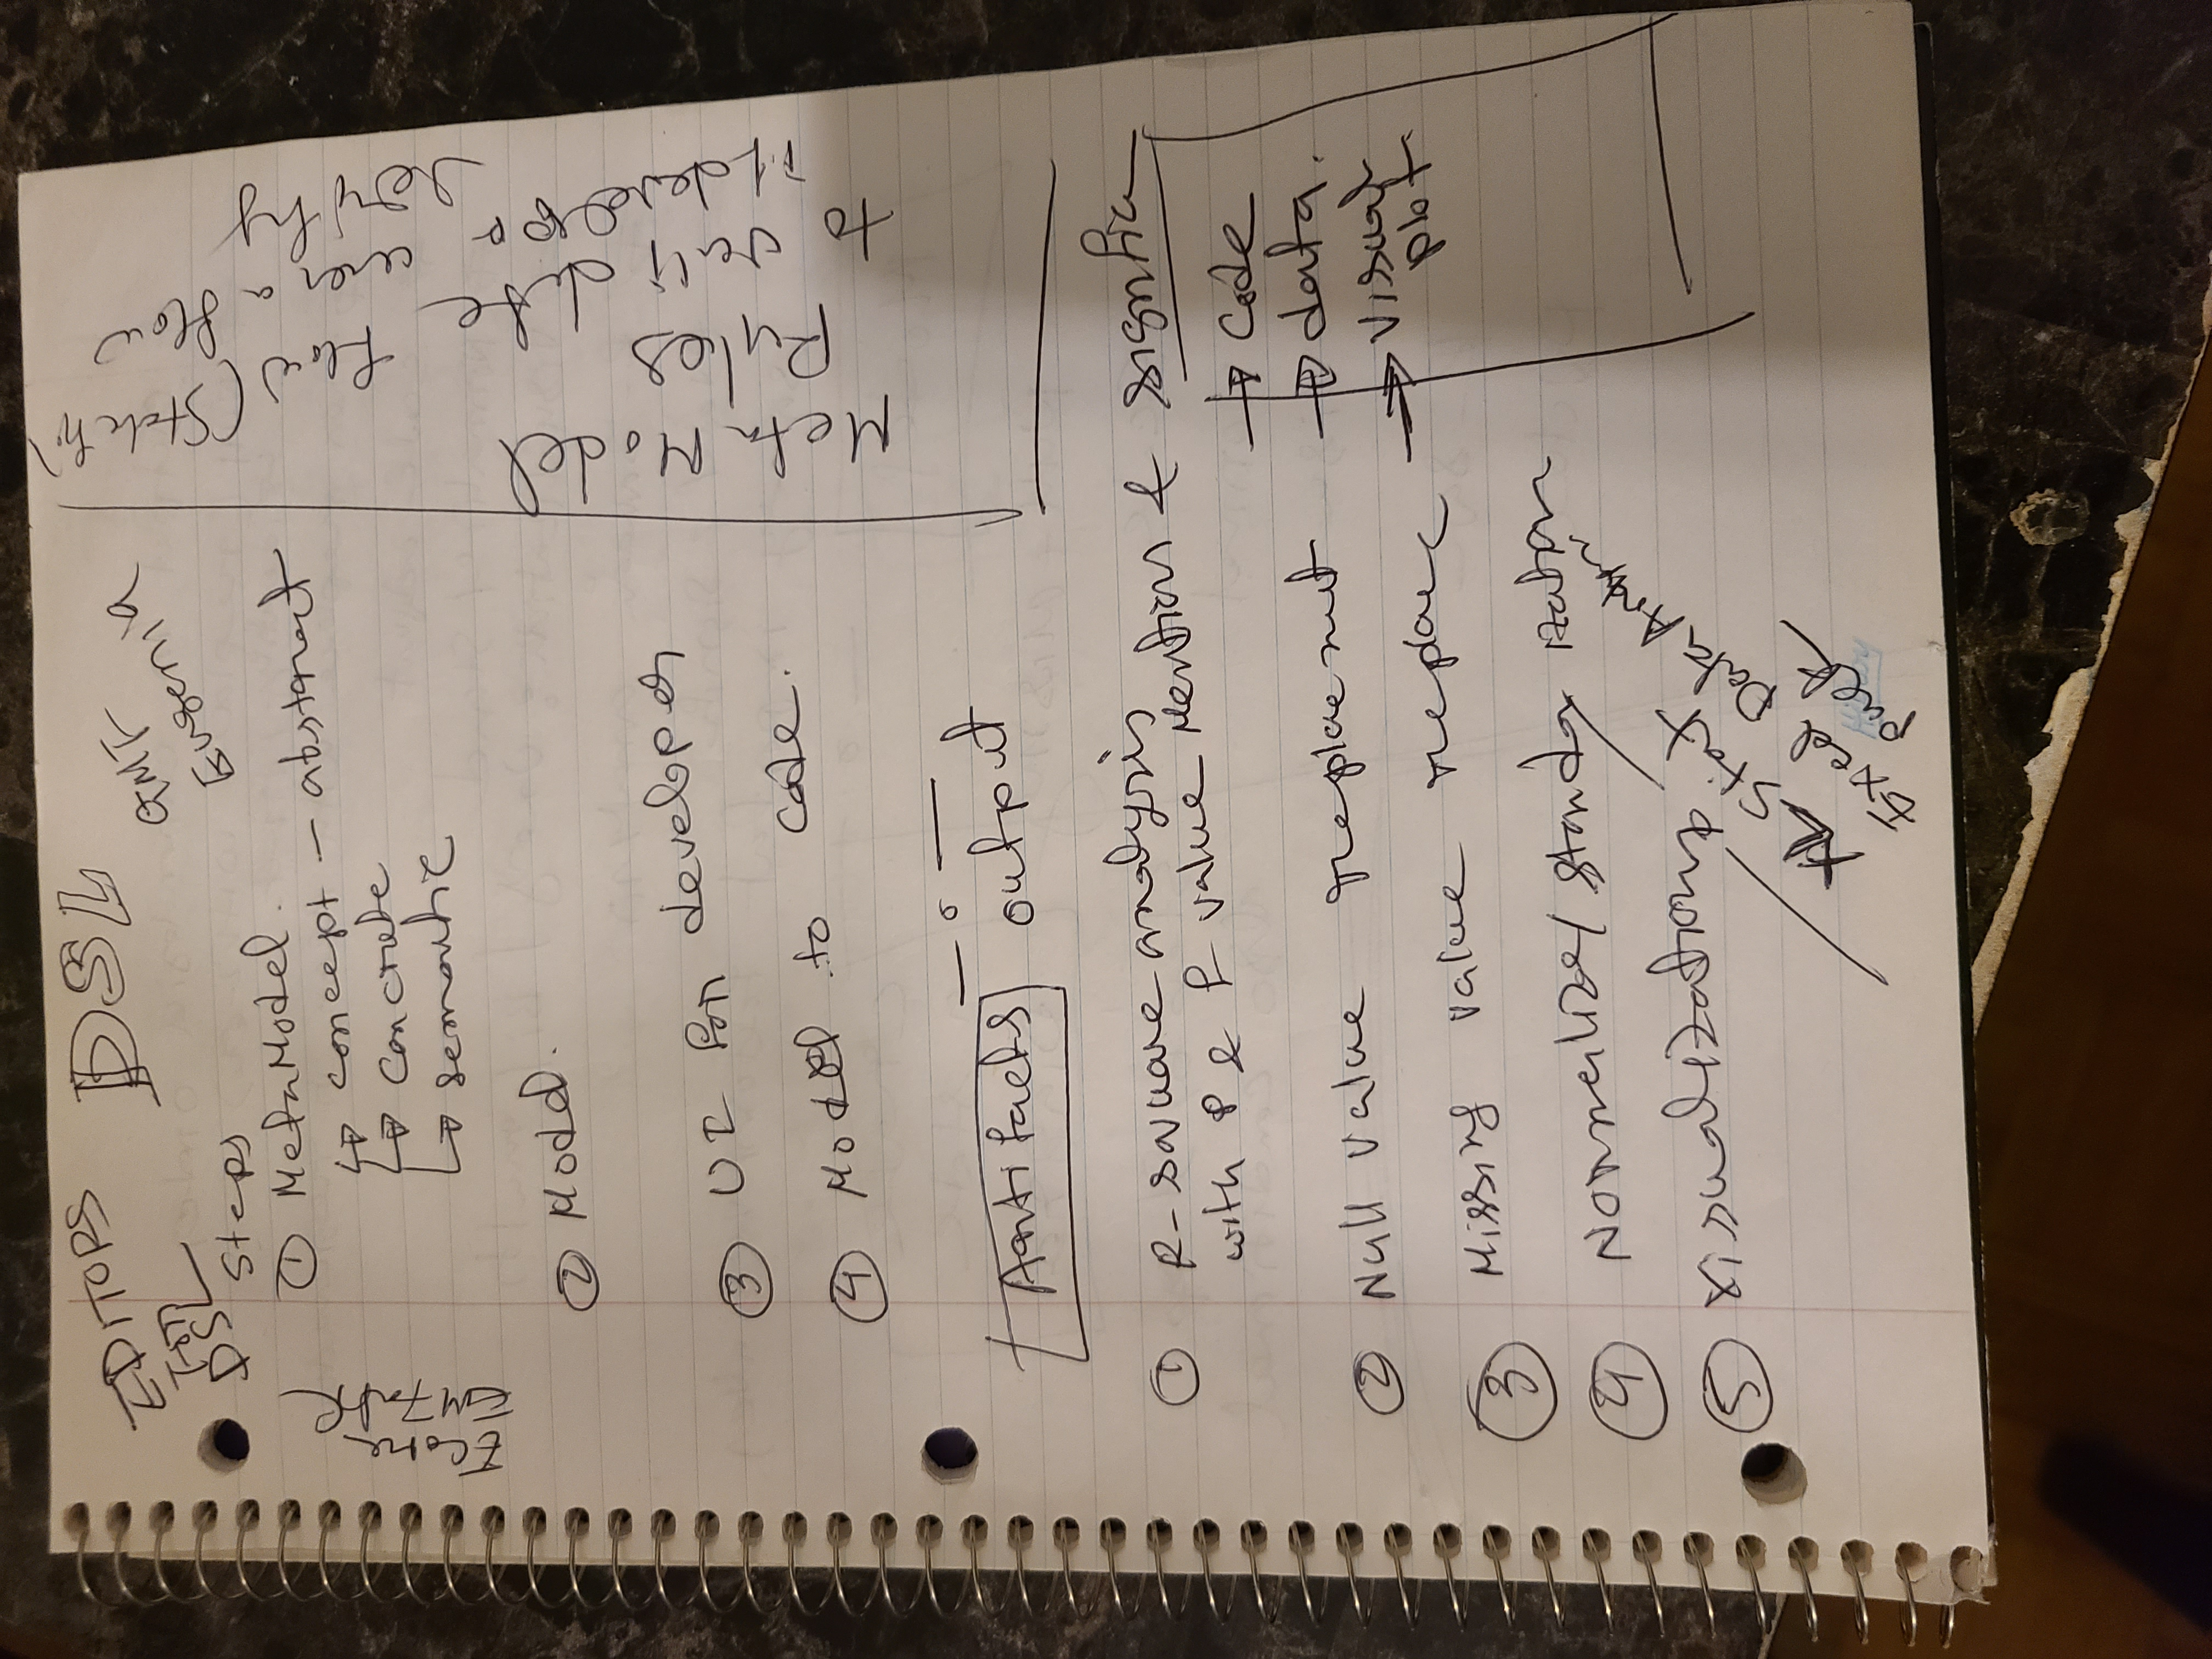
\includegraphics[scale=0.1, angle = -90]{sketch/1.jpg} \\
\hline
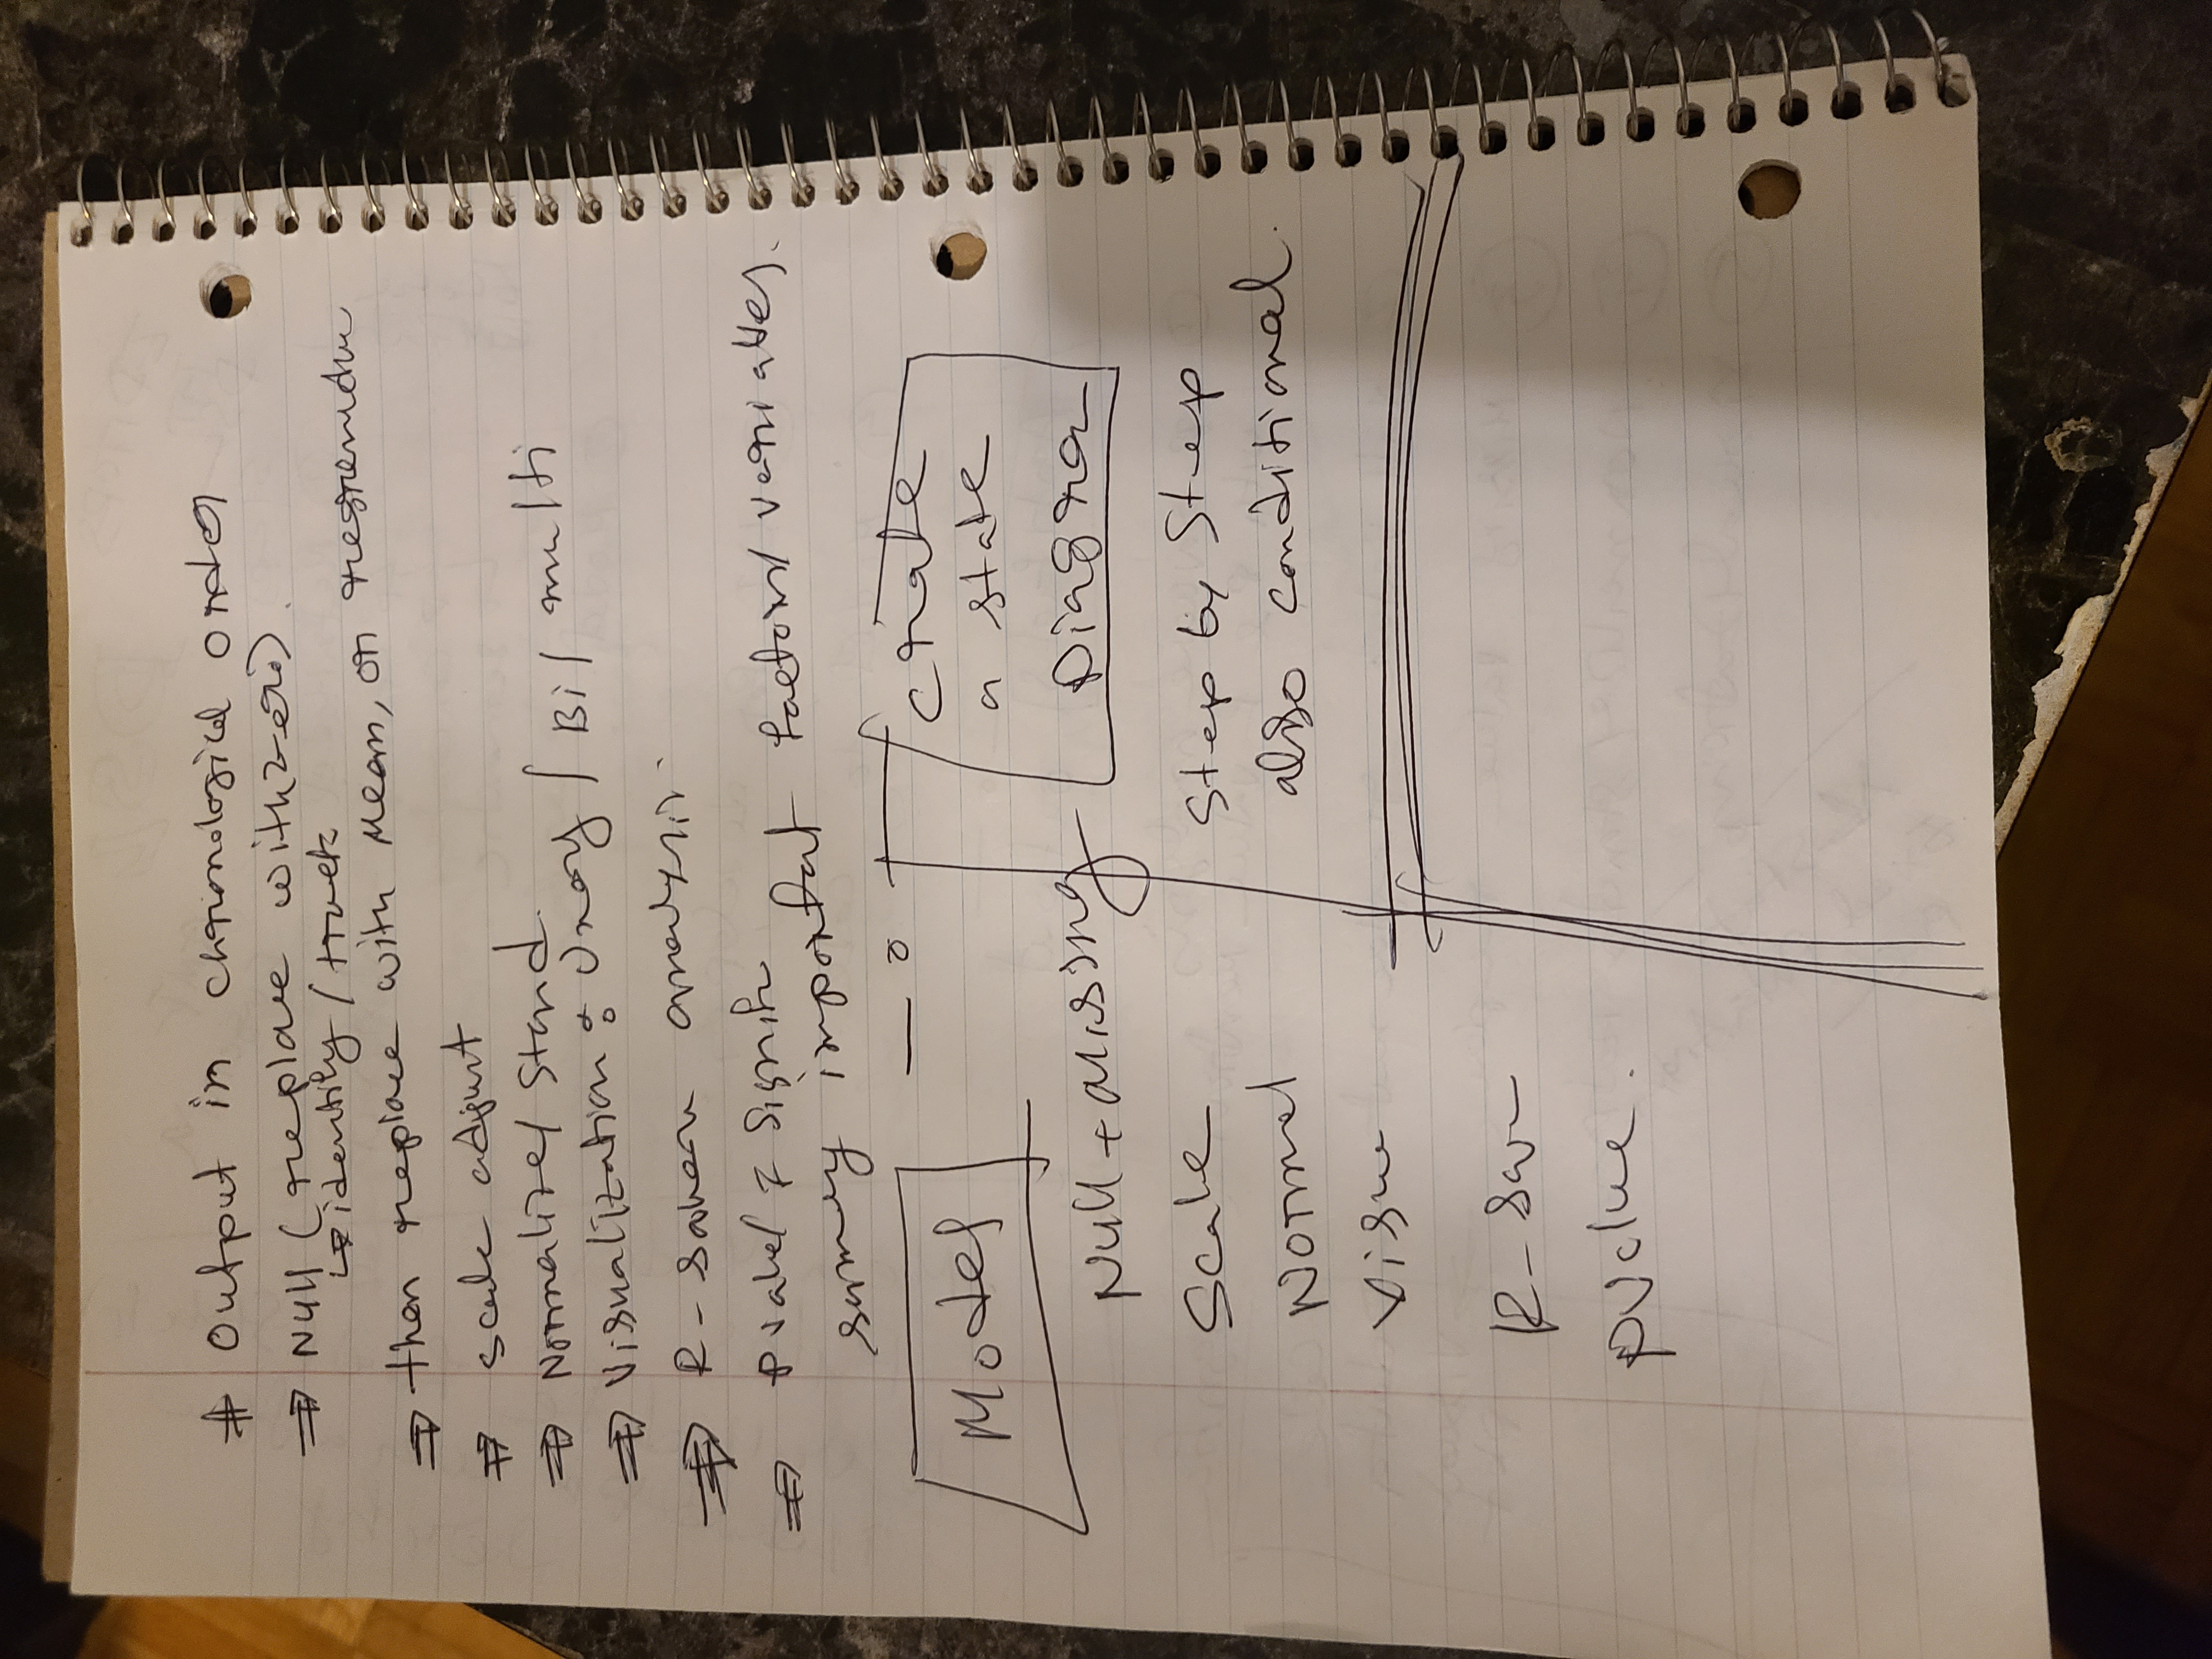
\includegraphics[scale=0.1, angle = -90]{sketch/2.jpg} \\
\hline
\end{tabular}

\begin{tabular}{|c|}
\hline
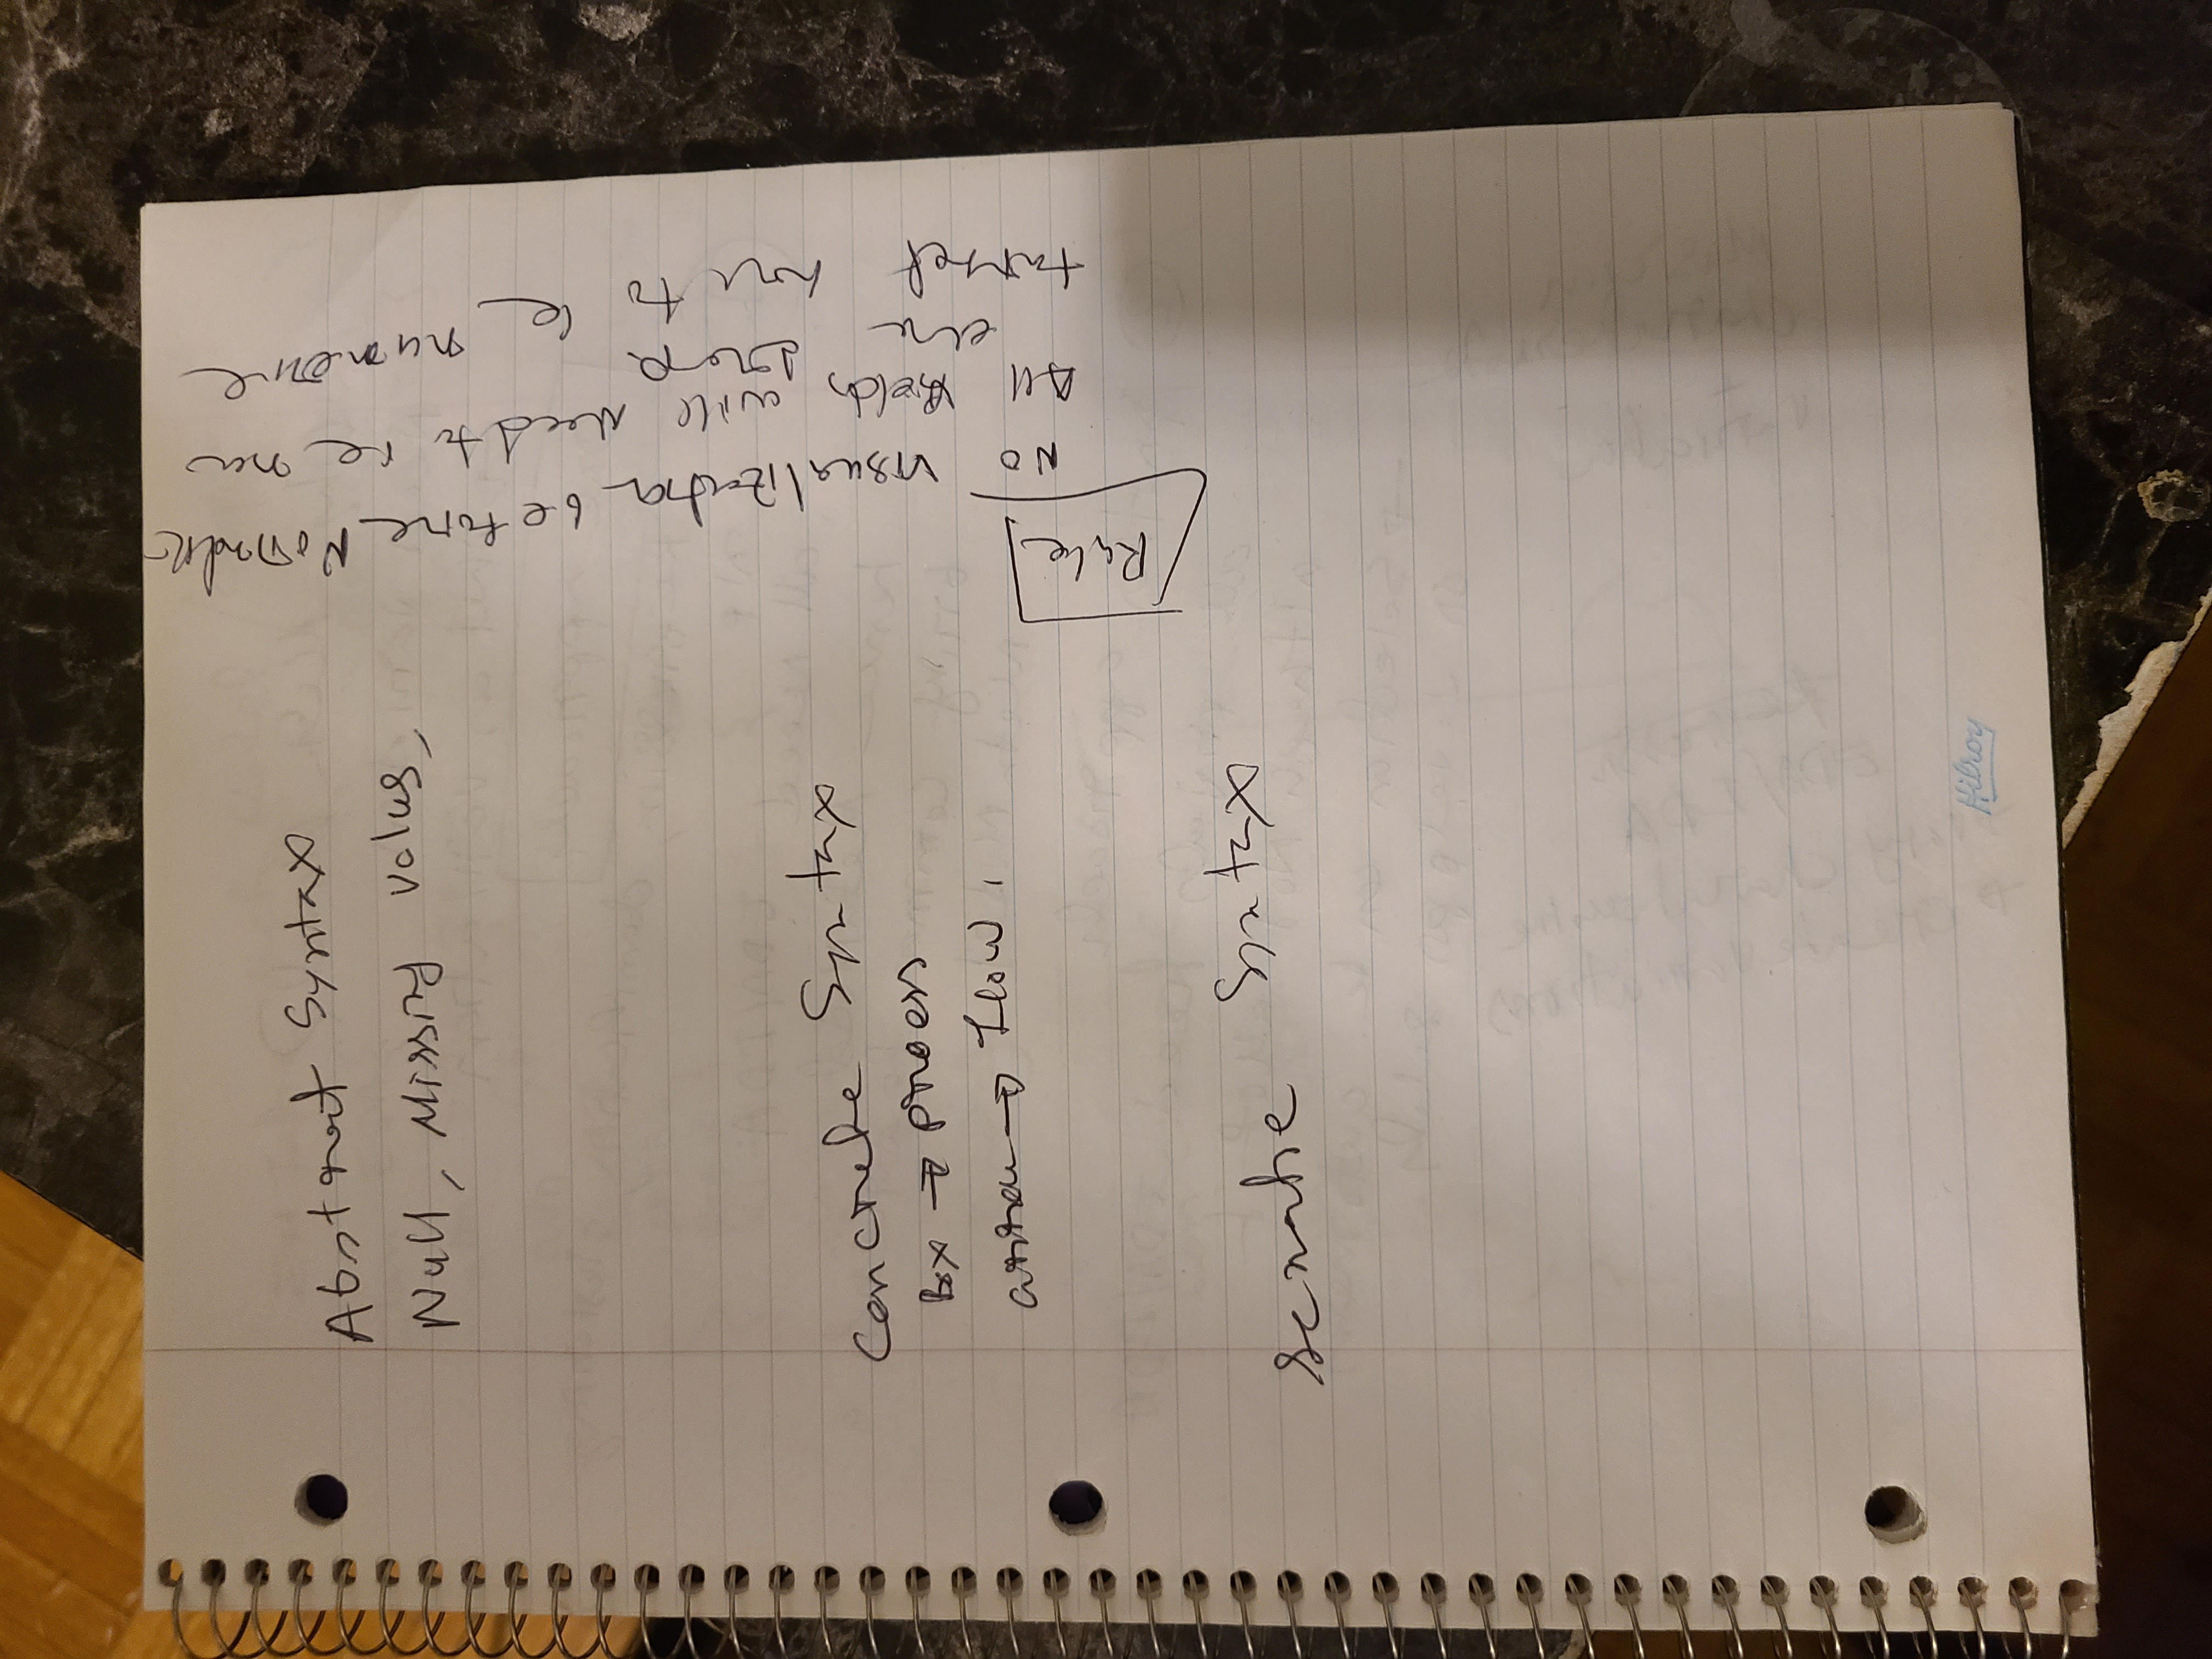
\includegraphics[scale=0.1, angle = -90]{sketch/3.jpg} \\
\hline
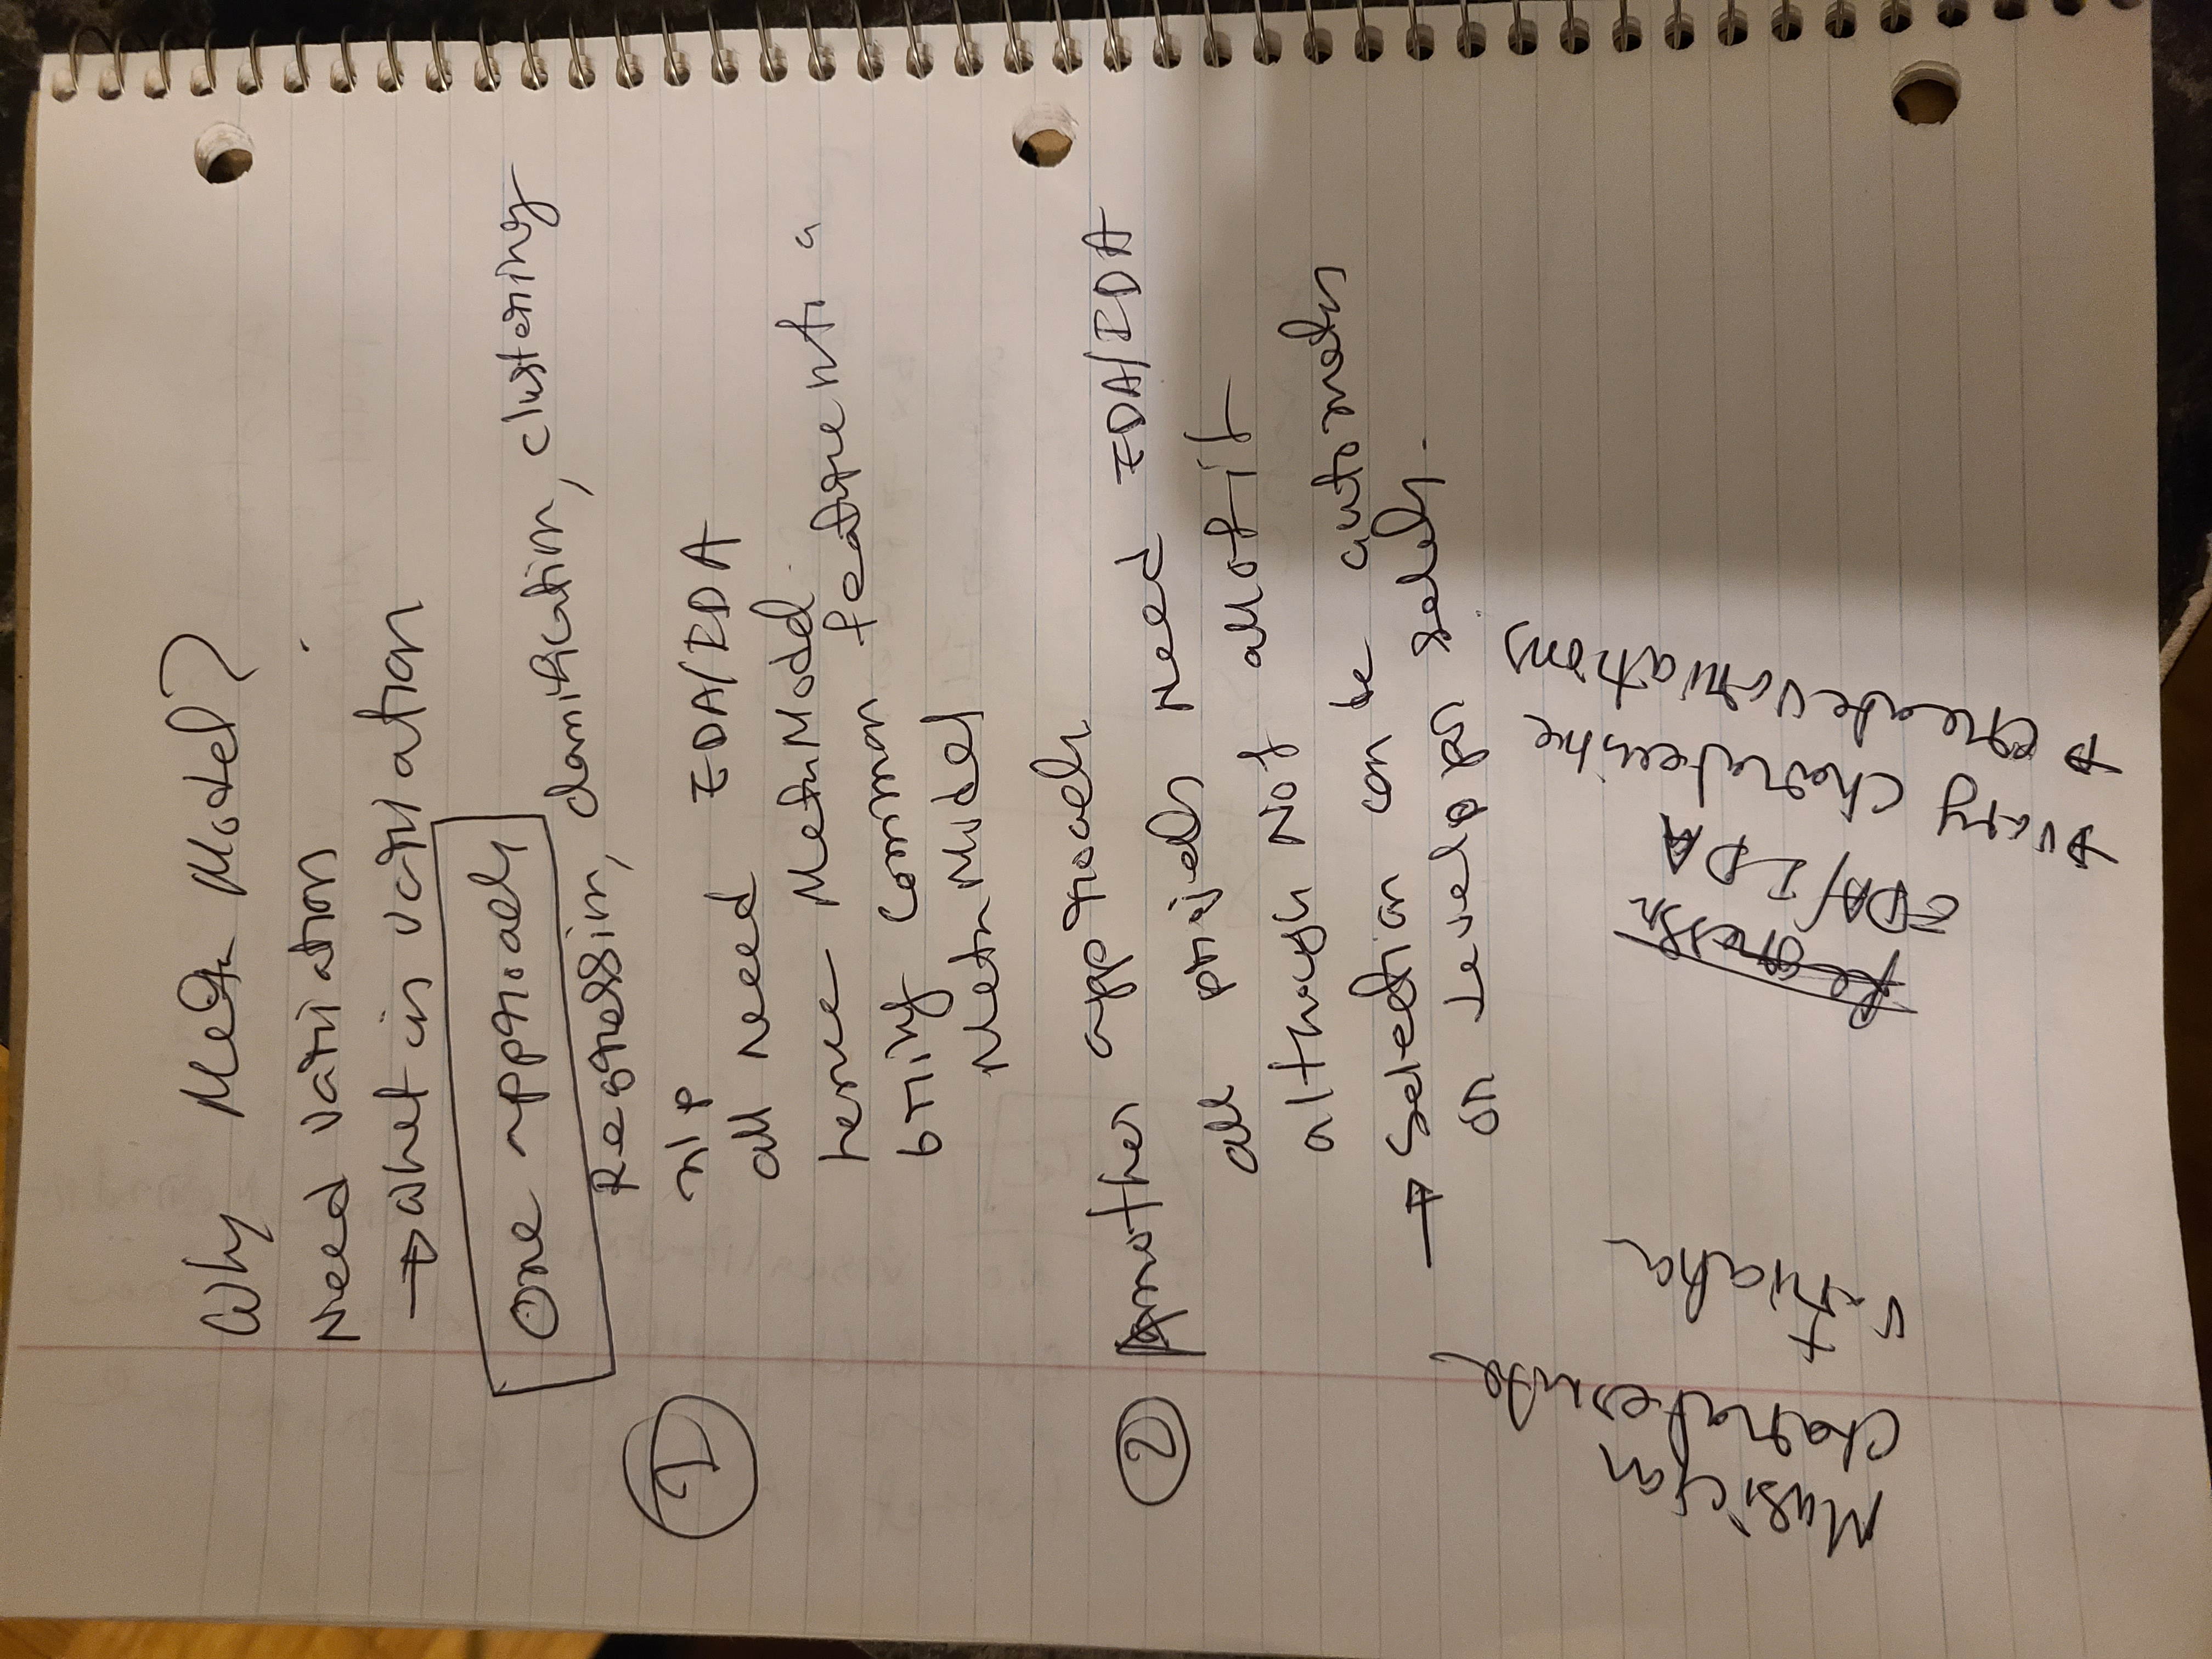
\includegraphics[scale=0.1, angle = -90]{sketch/4.jpg} \\
\hline
\end{tabular}

\begin{tabular}{|c|}
\hline
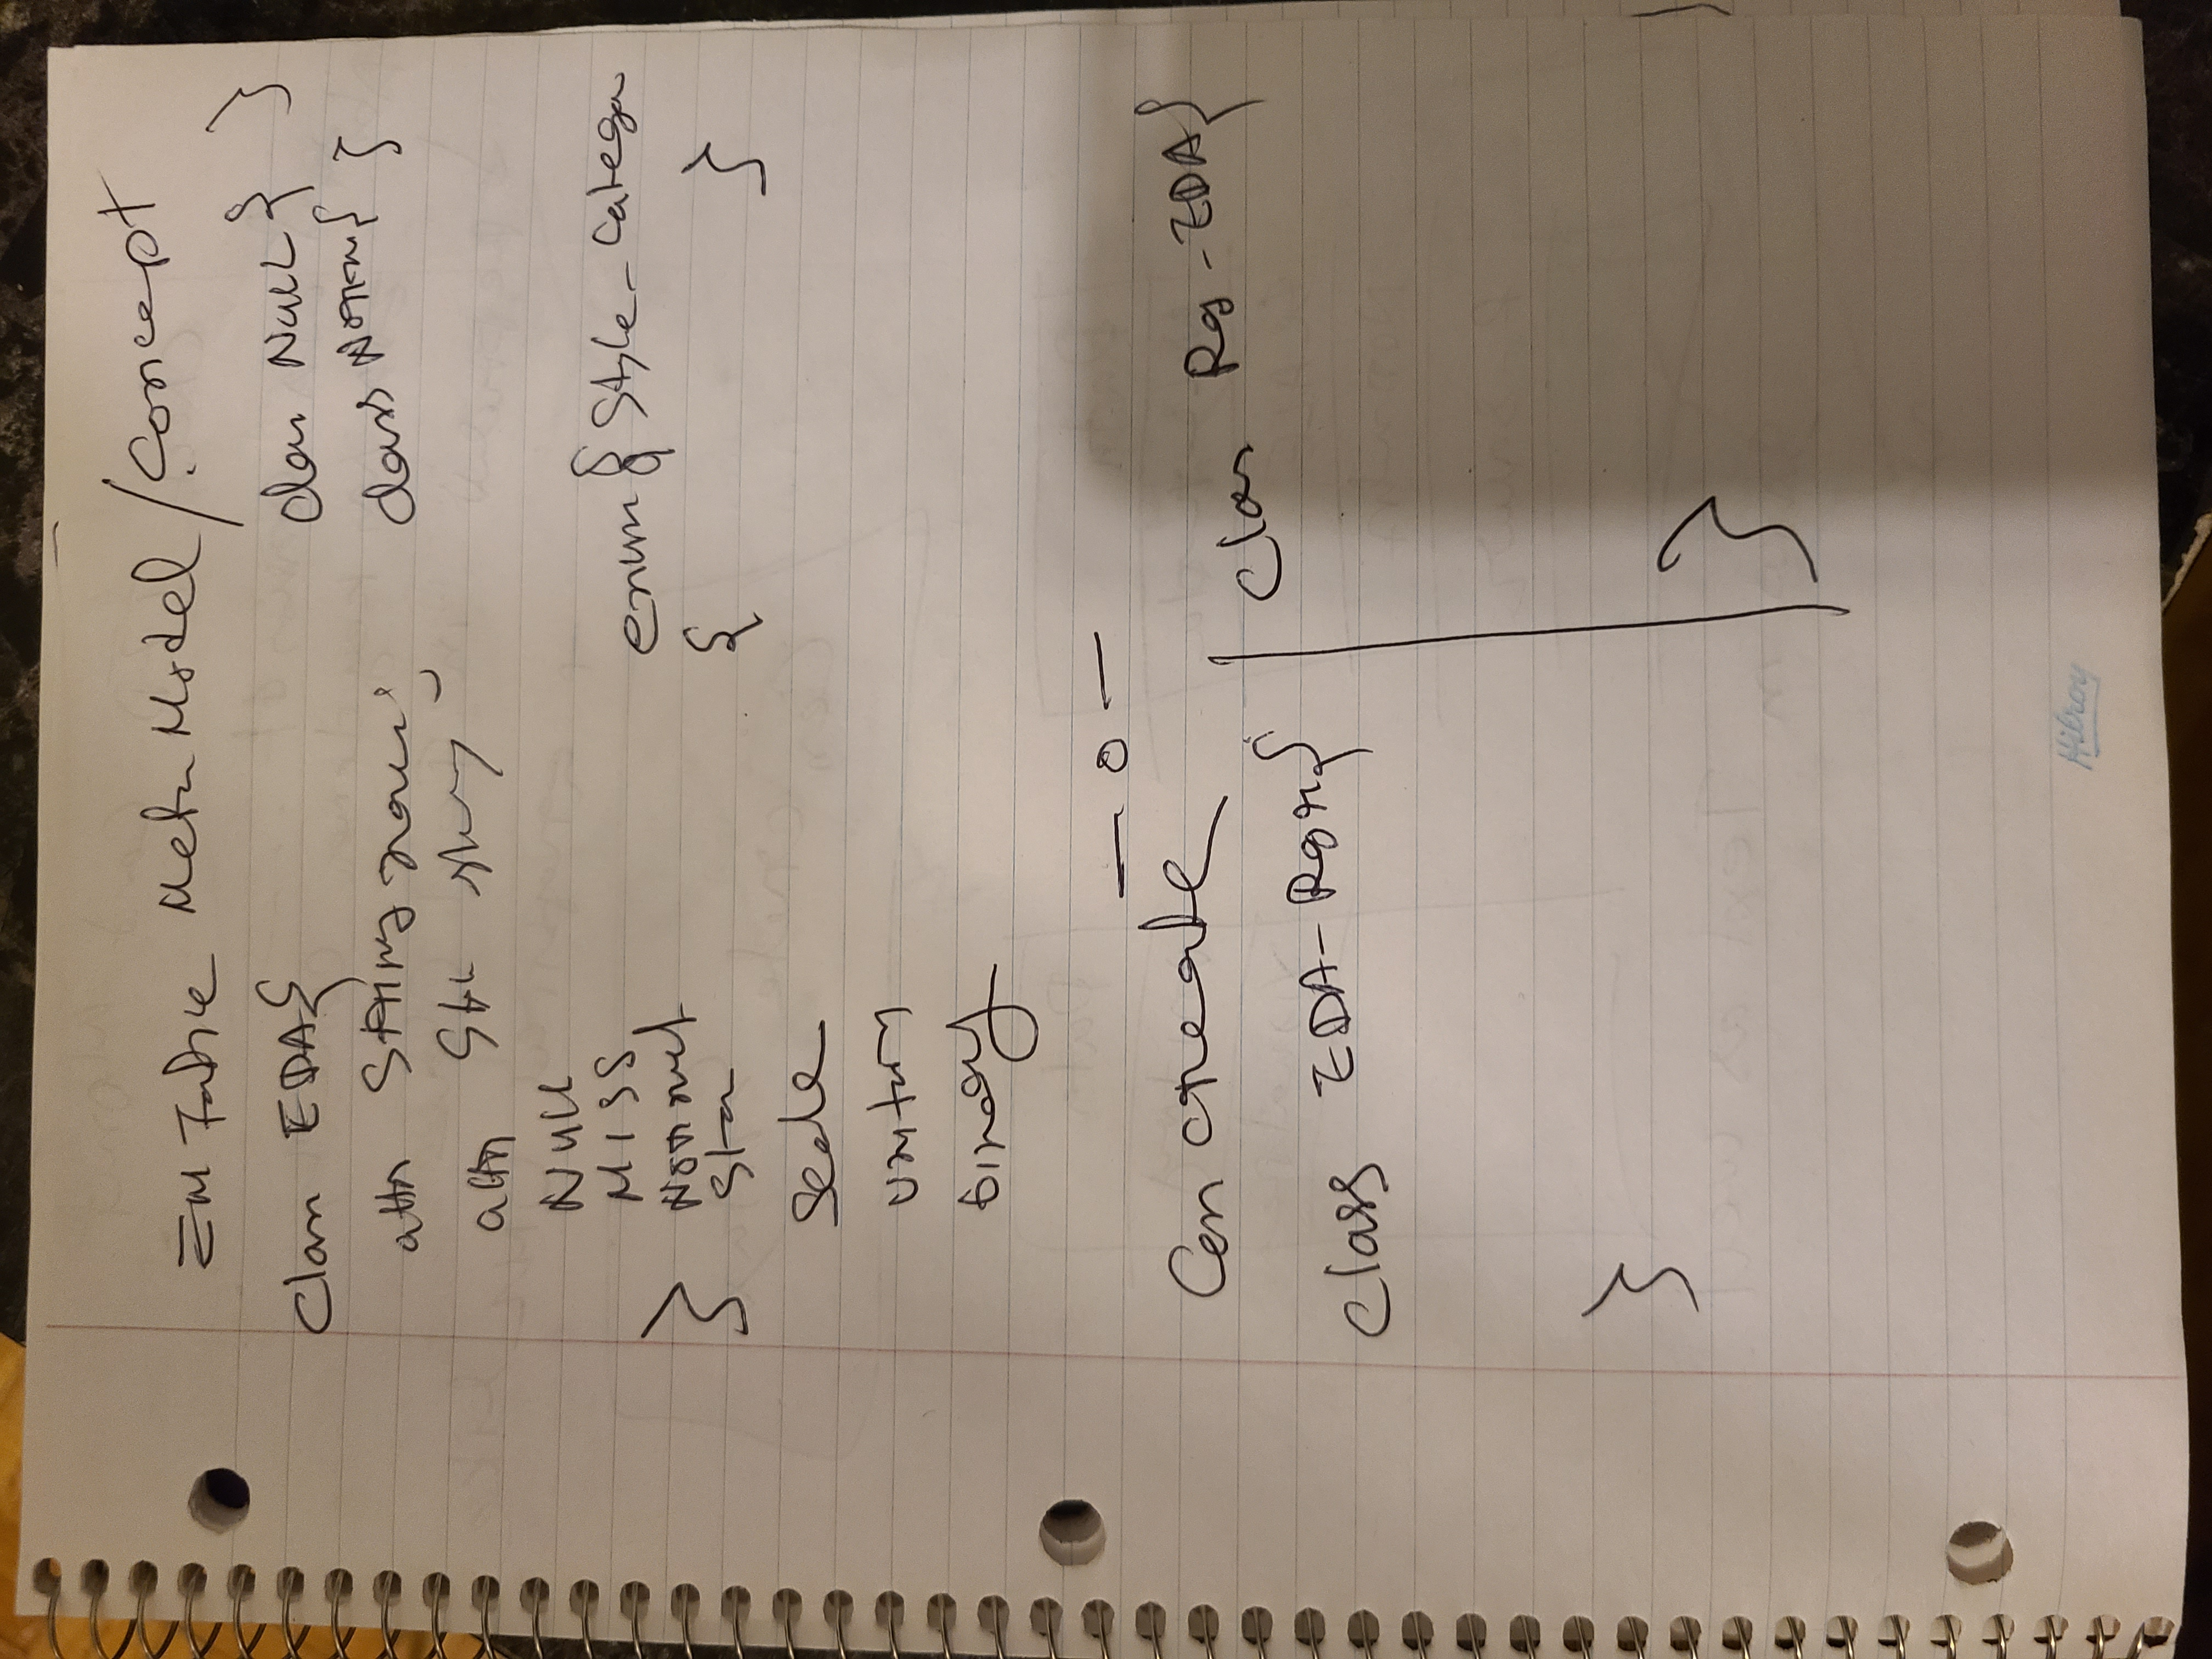
\includegraphics[scale=0.1, angle = -90]{sketch/5.jpg} \\ 
\hline
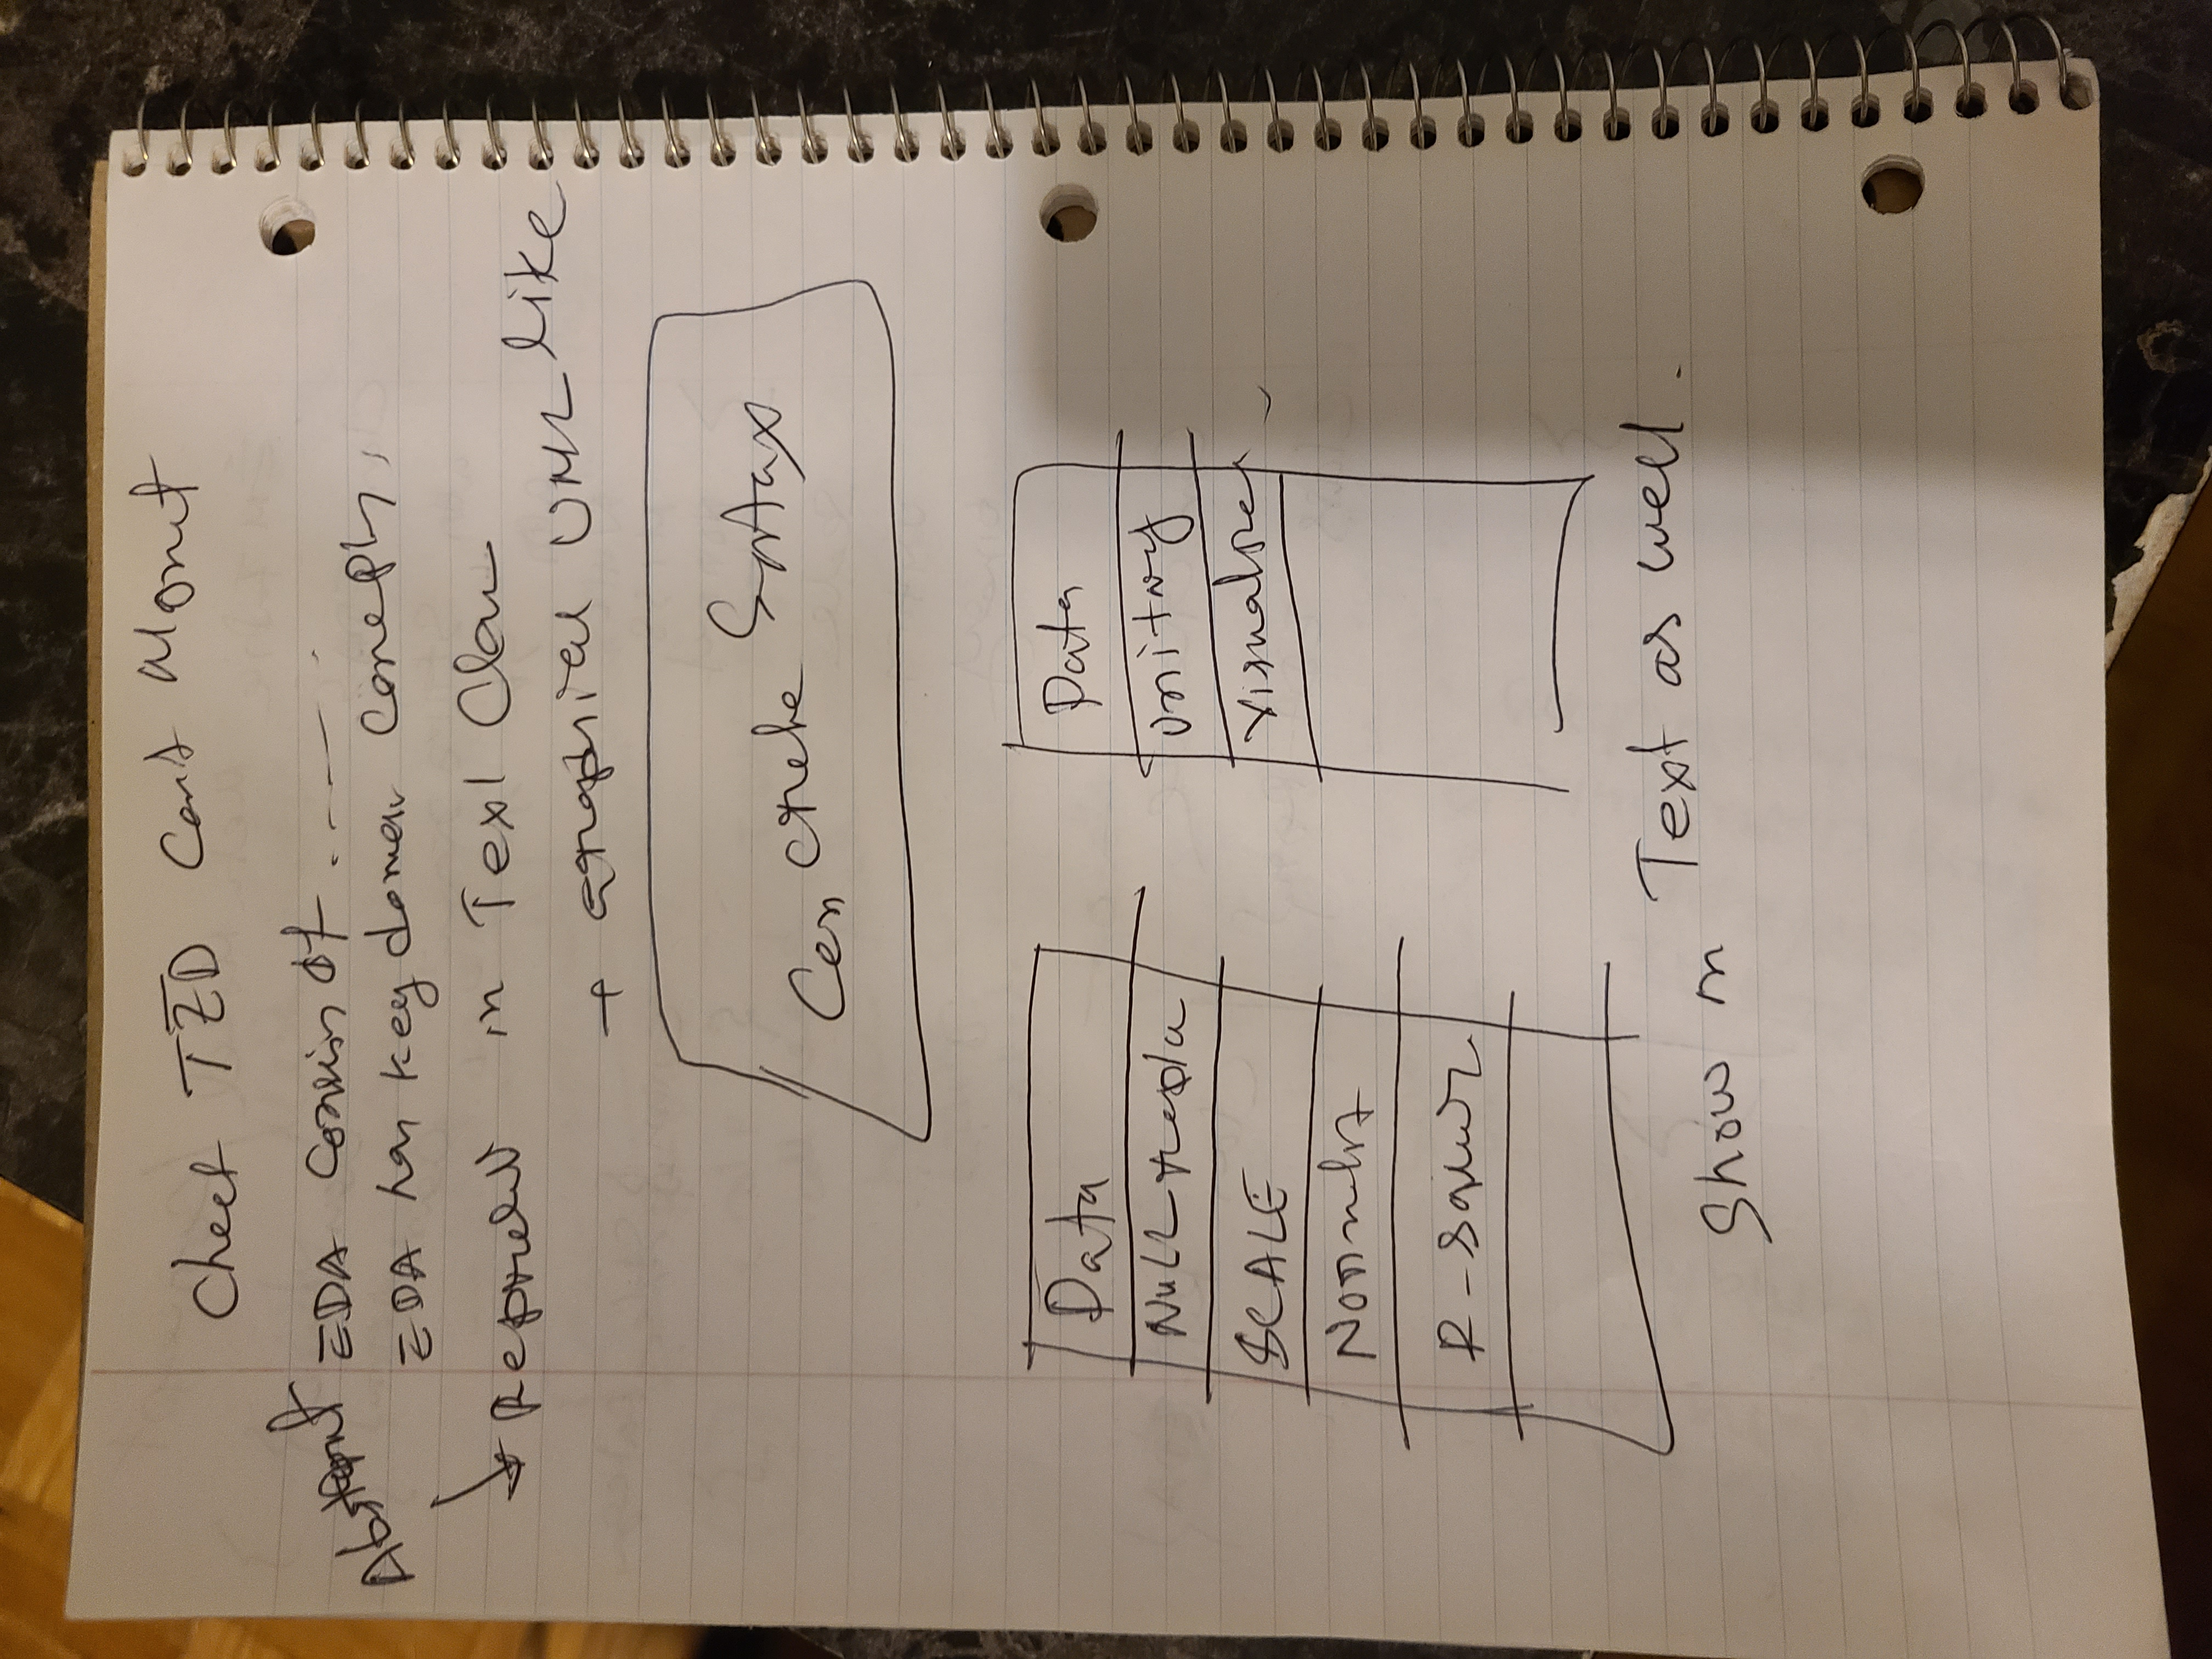
\includegraphics[scale=0.1, angle = -90]{sketch/6.jpg} \\
\hline
\end{tabular}


\begin{tabular}{|c|}
\hline
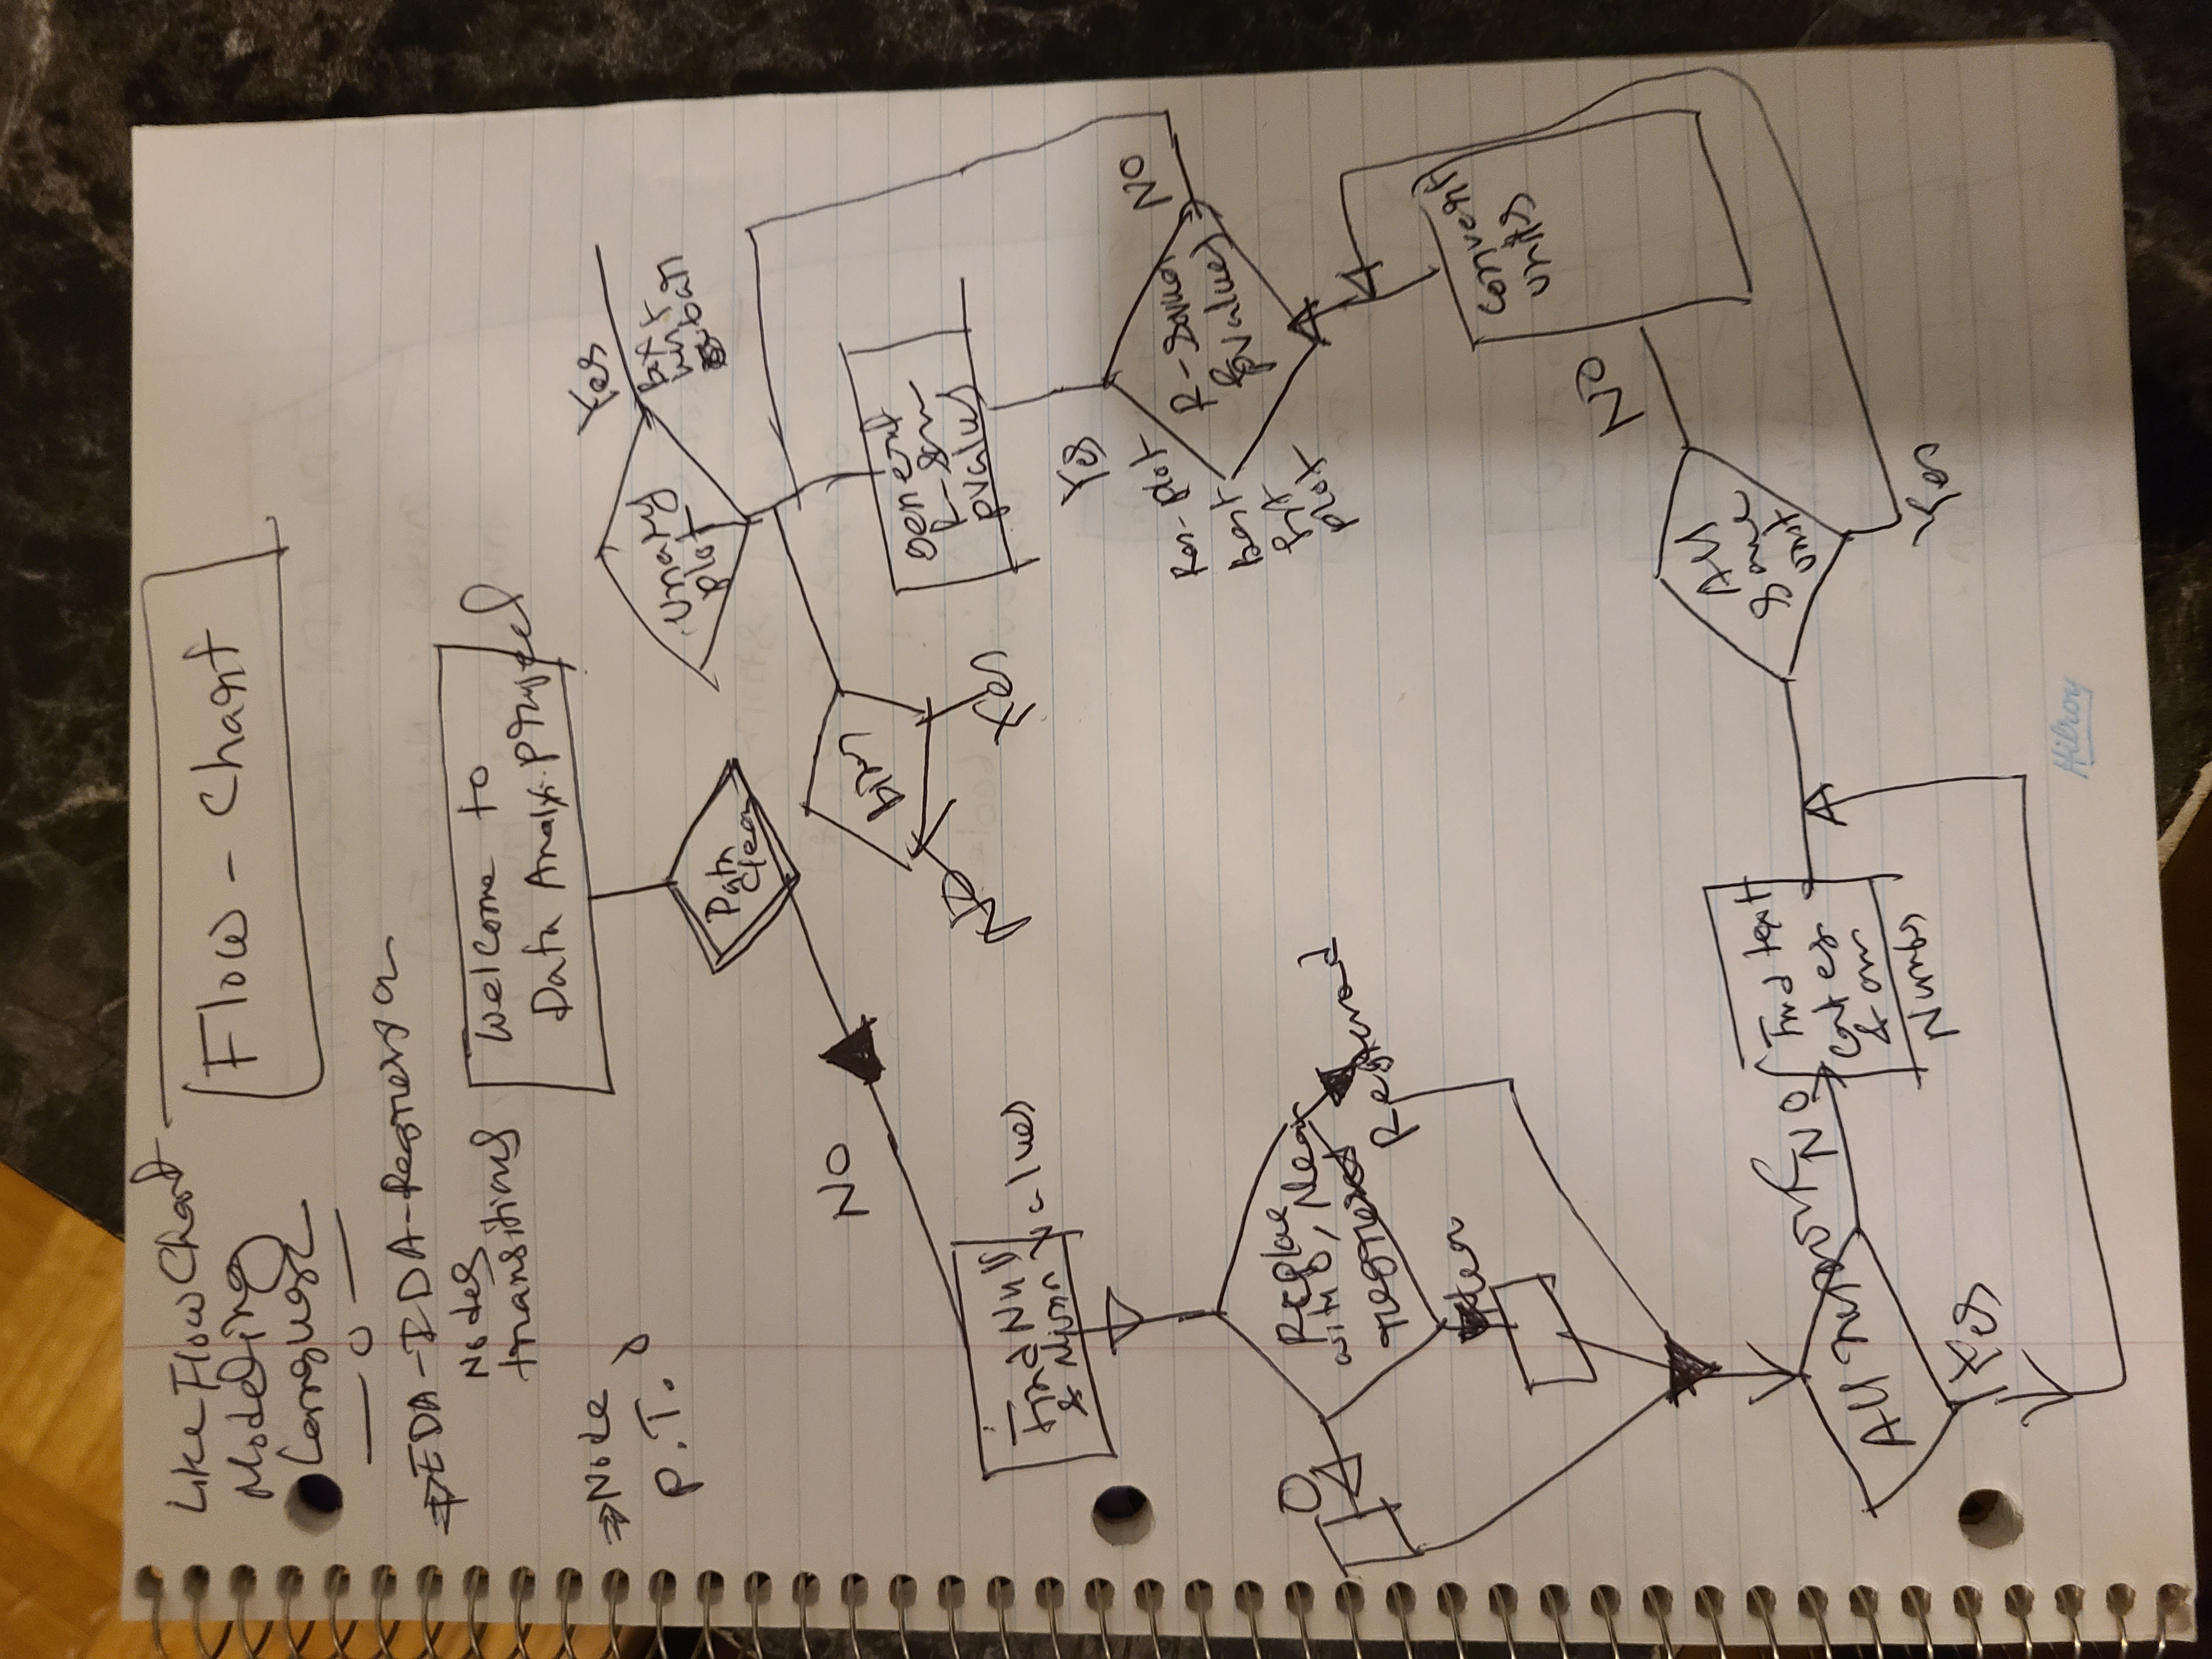
\includegraphics[scale=0.1, angle = -90]{sketch/7.jpg} \\ 
\hline
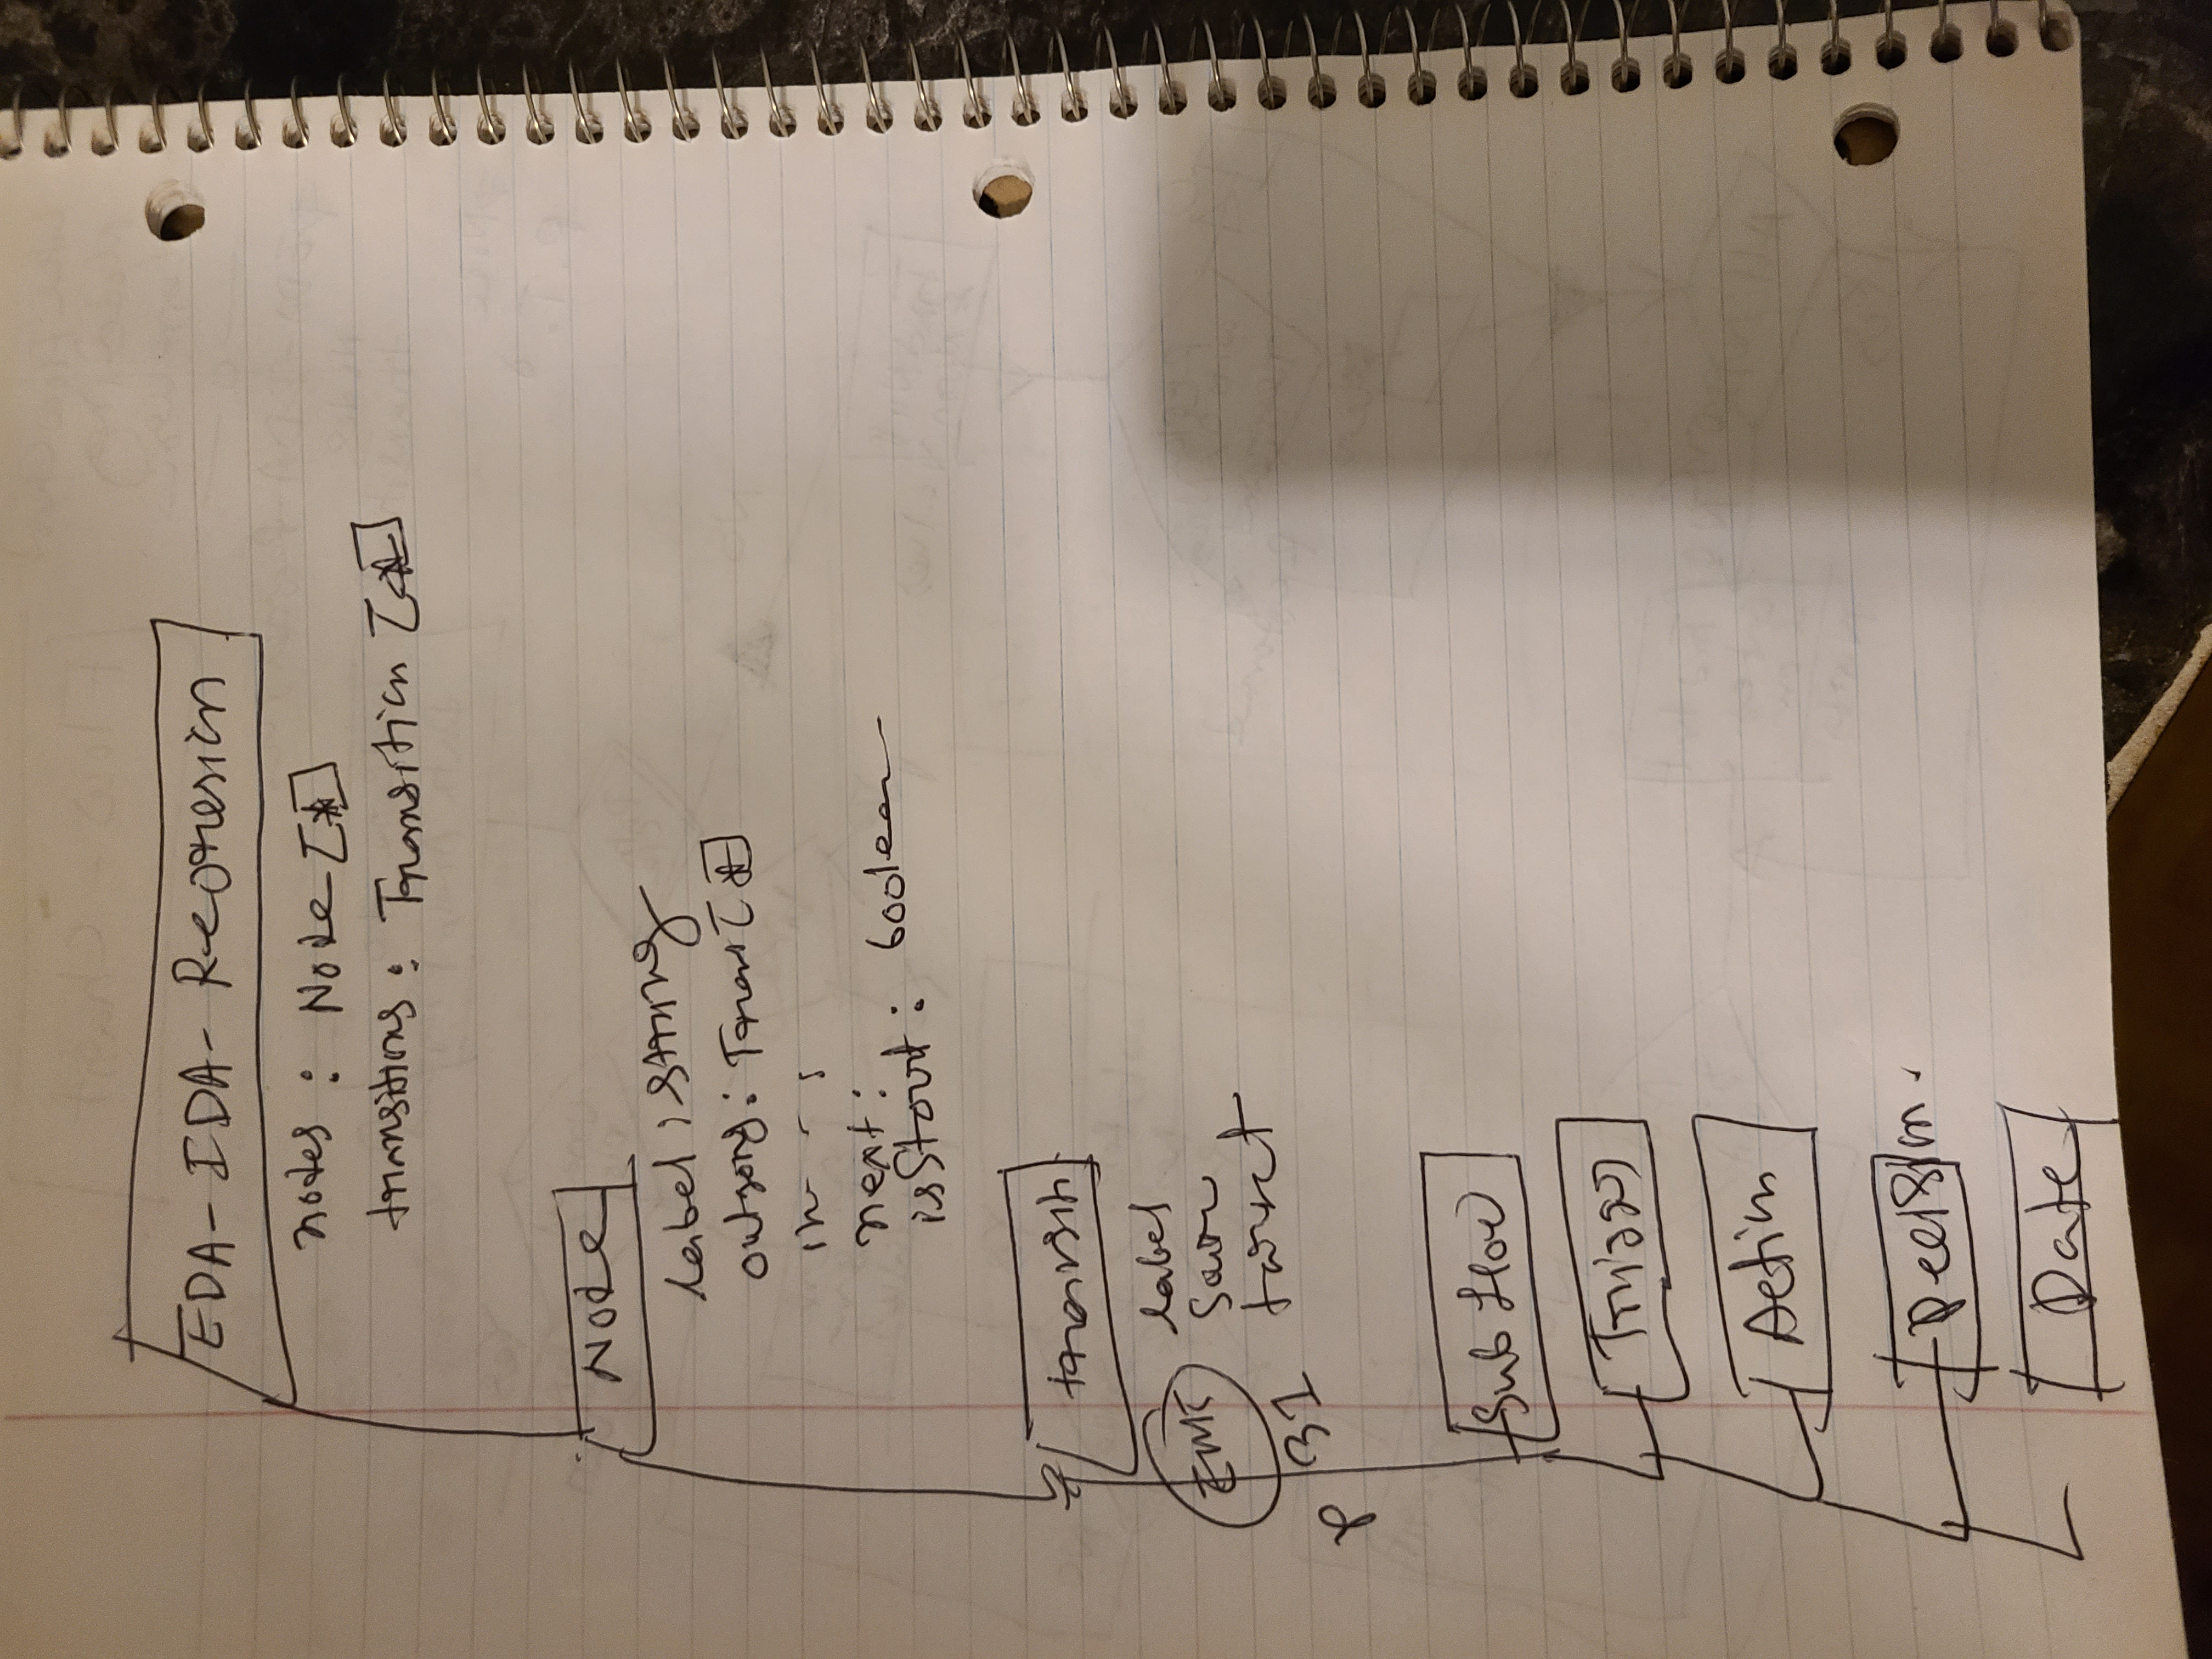
\includegraphics[scale=0.1, angle = -90]{sketch/8.jpg} \\
\hline
\end{tabular}
%\caption{Sketch of the Requirements and Plans}
%\label{sketch}
%\end{figure}
\end{document}